\documentclass{beamer}

\usepackage[mode=buildnew,subpreambles=true]{standalone}
\usetheme{Warsaw}

%%%%% PACKAGES

\usepackage{graphicx} % figures
\usepackage{multimedia} % videos
\usepackage{url}
\usepackage{amsmath}
\usepackage{amssymb}
\usepackage{mathrsfs}
\usepackage{mathtools}
\everymath{\displaystyle}
\usepackage{epstopdf} % conversion from .eps to .pdf
\usepackage[utf8]{inputenc}
\usepackage[T1]{fontenc}
\usepackage{upgreek}
\usepackage{nameref}
\usepackage{url}
\usepackage{pgf, tikz}
\usepackage{float}
\usepackage[english]{babel}
\usepackage[justification=justified]{caption}
\usepackage{subcaption}
\usepackage{xcolor,colortbl}
\usepackage{fontawesome}
\usepackage{tabularx}

\usepackage{biblatex}
\addbibresource{ref.bib}

%%%%% BEAMER TEMPLATE

%%%%%% Pink beamer colour theme
%% https://www.r-bloggers.com/create-your-own-beamer-template/

%%%% COLOURS

\definecolor{CaPink}{RGB}{232, 94, 138} % default pink
\definecolor{CaDarkUnsatPink}{RGB}{249, 26, 97} % dark unsaturated pink
\definecolor{CaLightPink}{RGB}{253, 175, 200} % light pink
\definecolor{CaRed}{RGB}{223, 47, 81} % red

%%%% THEME

%% header color
% https://tex.stackexchange.com/questions/321097/how-to-change-color-of-shadow-around-frametitle-latex-beamer
\pgfdeclarehorizontalshading[frametitle.bg,frametitle right.bg]{beamer@frametitleshade}{\paperheight}{
    color(0pt)=(CaPink);
    color(\paperwidth)=(CaRed)}

\setbeamercolor{normal text}{fg = black}

\setbeamercolor{frametitle}{fg = white, bg = CaPink}
\setbeamercolor{title}{fg = white, bg = CaPink}

\setbeamercolor{author in head/foot}{fg = white, bg = CaPink}
\setbeamercolor{title in head/foot}{fg = white, bg = CaRed}
\setbeamercolor{date in head/foot}{fg = white, bg = CaPink}

\setbeamercolor{section in toc}{fg = CaDarkUnsatPink}
\setbeamercolor{section in toc shaded}{fg = CaDarkUnsatPink}

\setbeamercolor{item}{fg = CaRed}
\setbeamercolor{subitem}{fg = CaPink}
\setbeamercolor{subsubitem}{fg = CaLightPink}
\setbeamercolor{description item}{fg = CaPink}

\setbeamercolor{bibliography entry author}{fg = CaPink}
\setbeamercolor{bibliography entry title}{fg = black}
\setbeamercolor{bibliography entry note}{fg = CaRed}

\setbeamercolor{footnote mark}{fg = CaRed}

\setbeamercolor{caption}{fg = white}
\setbeamercolor{caption name}{fg = CaPink}
\setbeamercolor{caption source}{fg = CaLightPink}

% % Standard block
% \setbeamercolor{block title}{fg = white, bg = green!20!blue}
% \setbeamercolor{block body}{bg = blue!1!white}
%
% % Alert block
% \setbeamercolor{block title alerted}{fg = white, bg = red}
% \setbeamercolor{block body alerted}{bg = red!1!white}
%
% % Example block
% \setbeamercolor{block title example}{fg = white, bg = green!80!blue}
% \setbeamercolor{block body example}{bg = green!1!white}
 % color theme

\setbeamerfont{frametitle}{size=\small}
\setbeamerfont{footnote}{size=\tiny}
\setbeamertemplate{headline}{} % clear header
\setbeamertemplate{navigation symbols}{} % remove buttons

\setbeamerfont{block title}{size=\tiny}
\setbeamerfont{block title example}{size=\tiny}
\setbeamerfont{block title alerted}{size=\tiny}

\setbeamersize{text margin left=3mm,text margin right=3mm}

\captionsetup{font=scriptsize,labelfont={scriptsize, color=CaPink, bf}}

% decrease space around math align environment
\newcommand{\zerodisplayskips}{%
  \setlength{\abovedisplayskip}{5pt}%
  \setlength{\belowdisplayskip}{5pt}%
  \setlength{\abovedisplayshortskip}{0pt}%
  \setlength{\belowdisplayshortskip}{0pt}}
\appto{\normalsize}{\zerodisplayskips}
\appto{\small}{\zerodisplayskips}
\appto{\footnotesize}{\zerodisplayskips}

% \AtBeginSubsection[]
% {
%  \begin{frame}<beamer>{}
%    \tableofcontents[currentsection,currentsubsection]
%  \end{frame}
% }
\AtBeginSection[]
{
{
\footerwithoutframenumber
  \begin{frame}<beamer>[noframenumbering]{Contents}
    \tableofcontents[currentsection]
  \end{frame}
}
}

\defbeamertemplate*{footline}{footer-framenumber}%
{  \begin{beamercolorbox}[ht=2.5ex]{bordure}
\begin{beamercolorbox}[wd=0.2\paperwidth,ht=2.5ex,dp=1ex,center]{author in head/foot}%
\usebeamerfont{author in head}\insertshortauthor
\end{beamercolorbox}%
\begin{beamercolorbox}[wd=0.57\paperwidth,ht=2.5ex,dp=1ex,center]{title in head/foot}%
\usebeamerfont{title in head/foot}\insertshorttitle
\end{beamercolorbox}%
\begin{beamercolorbox}[wd=0.12\paperwidth,ht=2.5ex,dp=1ex,center]{title in head/foot}%
\usebeamerfont{title in head/foot}\insertdate
\end{beamercolorbox}%
\begin{beamercolorbox}[wd=0.11\paperwidth,ht=2.5ex,dp=1ex,center]{date in head/foot}%
\usebeamerfont{date in head/foot}\insertframenumber /\inserttotalframenumber{}\hspace{2ex}
\end{beamercolorbox}%

  \end{beamercolorbox}
}

\providecommand{\footerwithoutframenumber}[0]{
\setbeamertemplate{footline}%
{  \begin{beamercolorbox}[ht=2.5ex]{bordure}
\begin{beamercolorbox}[wd=0.2\paperwidth,ht=2.5ex,dp=1ex,center]{author in head/foot}%
\usebeamerfont{author in head}\insertshortauthor
\end{beamercolorbox}%
\begin{beamercolorbox}[wd=0.57\paperwidth,ht=2.5ex,dp=1ex,center]{title in head/foot}%
\usebeamerfont{title in head/foot}\insertshorttitle
\end{beamercolorbox}%
\begin{beamercolorbox}[wd=0.12\paperwidth,ht=2.5ex,dp=1ex,center]{title in head/foot}%
\usebeamerfont{title in head/foot}\insertdate
\end{beamercolorbox}%
\begin{beamercolorbox}[wd=0.11\paperwidth,ht=2.5ex,dp=1ex,center]{date in head/foot}%
\usebeamerfont{date in head/foot} % \RomanNumeralCaps{\insertsectionnumber}
\end{beamercolorbox}%

  \end{beamercolorbox}
}
}

% \defbeamertemplate*{headline}{mytheme}%
% {  \begin{beamercolorbox}[ht=2.5ex]{bordure}
% \begin{beamercolorbox}[wd=\paperwidth,ht=2.5ex,dp=2ex]{author in head/foot}%
% \usebeamerfont{author in head}\vskip6pt\insertsectionnumber.~\insertsection \hfill \insertsubsection
% \end{beamercolorbox}%
%
%   \end{beamercolorbox}
% }

\makeatletter
\let\insertsupervisor\relax
\newcommand\supervisortitle{supervised by}
\mode<all>
{
  \newcommand\supervisor[1]{\def\insertsupervisor{#1}}
  \titlegraphic{}
}
\let\insertlocation\relax
\mode<all>
{
  \newcommand\location[1]{\def\insertlocation{#1}}
  \titlegraphic{}
}
\let\insertshorttitle\relax
\mode<all>
{
  \newcommand\shorttitle[1]{\def\insertshorttitle{#1}}
  \titlegraphic{}
}
\defbeamertemplate*{title page}{supdefault}[1][]
{
  \vbox{}
  \vfill
  \begingroup
    \centering
    \hfill
    \begin{beamercolorbox}[wd=0.80\paperwidth,sep=8pt,center,#1]{title}
      \usebeamerfont{title}\inserttitle\par%
      \ifx\insertsubtitle\@empty\relax%
      \else%
        \vskip0.25em%
        {\usebeamerfont{subtitle}\usebeamercolor[fg]{subtitle}\insertsubtitle\par}%
      \fi%
    \end{beamercolorbox}%
    \hfill\hfill
    \vskip1em\par
    \vspace{-10pt}
    \begin{beamercolorbox}[sep=8pt,center,#1]{author}
      \usebeamerfont{author}\textbf{\insertauthor}
    \end{beamercolorbox}
    \ifx\insertlocation\relax\relax\else
    \vspace{-10pt}
    \begin{beamercolorbox}[sep=8pt,center,#1]{author}
      \usebeamerfont{author}{\footnotesize \supervisortitle}~{\small\insertsupervisor}
    \end{beamercolorbox}\fi
    \vspace{-5pt}
    \ifx\insertlocation\relax\relax\else
    \begin{beamercolorbox}[sep=8pt,center,#1]{author}
      \usebeamerfont{author}{\small\insertlocation}
    \end{beamercolorbox}\fi
    \vspace{-10pt}
    \begin{beamercolorbox}[sep=8pt,center,#1]{date}
      \usebeamerfont{date}{\footnotesize \insertdate}
    \end{beamercolorbox}\vskip0.5em
    {\usebeamercolor[fg]{titlegraphic}\inserttitlegraphic\par}
  \endgroup
  \vfill
}
\setbeamertemplate{title page}[supdefault][colsep=-4bp,rounded=true,shadow=\beamer@themerounded@shadow]\makeatother

\makeatletter
\newlength\beamerleftmargin
\setlength\beamerleftmargin{\Gm@lmargin}
\makeatother

%%%%% MACROS

\providecommand{\insertmovie}[4]{
\begin{figure}[h!]
  \centering
  \Movie{#1}{#2}{#3}
  \ifblank{#4}{}{\caption{\textit{(Movie)} #4}}
\end{figure}
}

\providecommand{\Movie}[3]{
  \movie[width=#1\linewidth]{\includegraphics[width=#1\linewidth]{#2}}{#3}
}

\providecommand{\inserttikz}[2]{
\begin{figure}[h!]
  \centering
  \includestandalone{figures/tikz/#1}
  \ifblank{#2}{}{\caption{#2}}
\end{figure}
}

\providecommand{\RomanNumeralCaps}[1]
    {\MakeUppercase{\romannumeral #1}}

\providecommand{\return}[0]{\mbox{}\\}

\providecommand{\FigureFrom}[2]{
  [{\usebeamercolor[fg]{caption source} from:} \fullcite{#1}\ifblank{#2}{}{ (Fig.~#2)}]
}

\newrobustcmd*{\footfullcitenomark}{%
  \AtNextCite{%
    \let\thefootnote\relax
    \let\mkbibfootnote\mkbibfootnotetext}%
  \footfullcite}

\providecommand\footnotenomark[1]{%
  \begingroup
  \renewcommand\thefootnote{}\footnote{#1}%
  \addtocounter{footnote}{-1}%
  \endgroup
}

% \makeatletter
% \providecommand{\xRightarrow}[2][]{\ext@arrow 0359\Rightarrowfill@{#1}{#2}}
% \makeatother


%%%%% INFORMATION

\title{Dense active Ornstein-Uhlenbeck particles}
\shorttitle{Dense AOUPs}

\author{Yann-Edwin Keta}

\location{}

\supervisor{Ludovic Berthier and Robert Jack}

\date{02/02/2021}

%%%%% DOCUMENT

\begin{document}

%% TITLE PAGE

{
\setbeamertemplate{footline}{}
\makeatletter
    \setbeamertemplate{headline}[default]
    \def\beamer@entrycode{\vspace*{-\headheight}}
\begin{frame}[noframenumbering]

\titlepage

\end{frame}
}

%% TABLE OF CONTENTS

{\footerwithoutframenumber
\begin{frame}<beamer>[noframenumbering]{Contents}
  \tableofcontents
\end{frame}
}

%% PRESENTATION

\section{Motivation and model}

\begin{frame}{Motivation}

\begin{itemize}
  \item Both high $\phi$ and $\tau_p$ not well explored.
  \item Theories of active glass transition for AOUPs focus on low $\tau_p$.
  \item Evidence for lare scale velocity correlations in the active liquid.
\end{itemize}

\begin{figure}
\centering
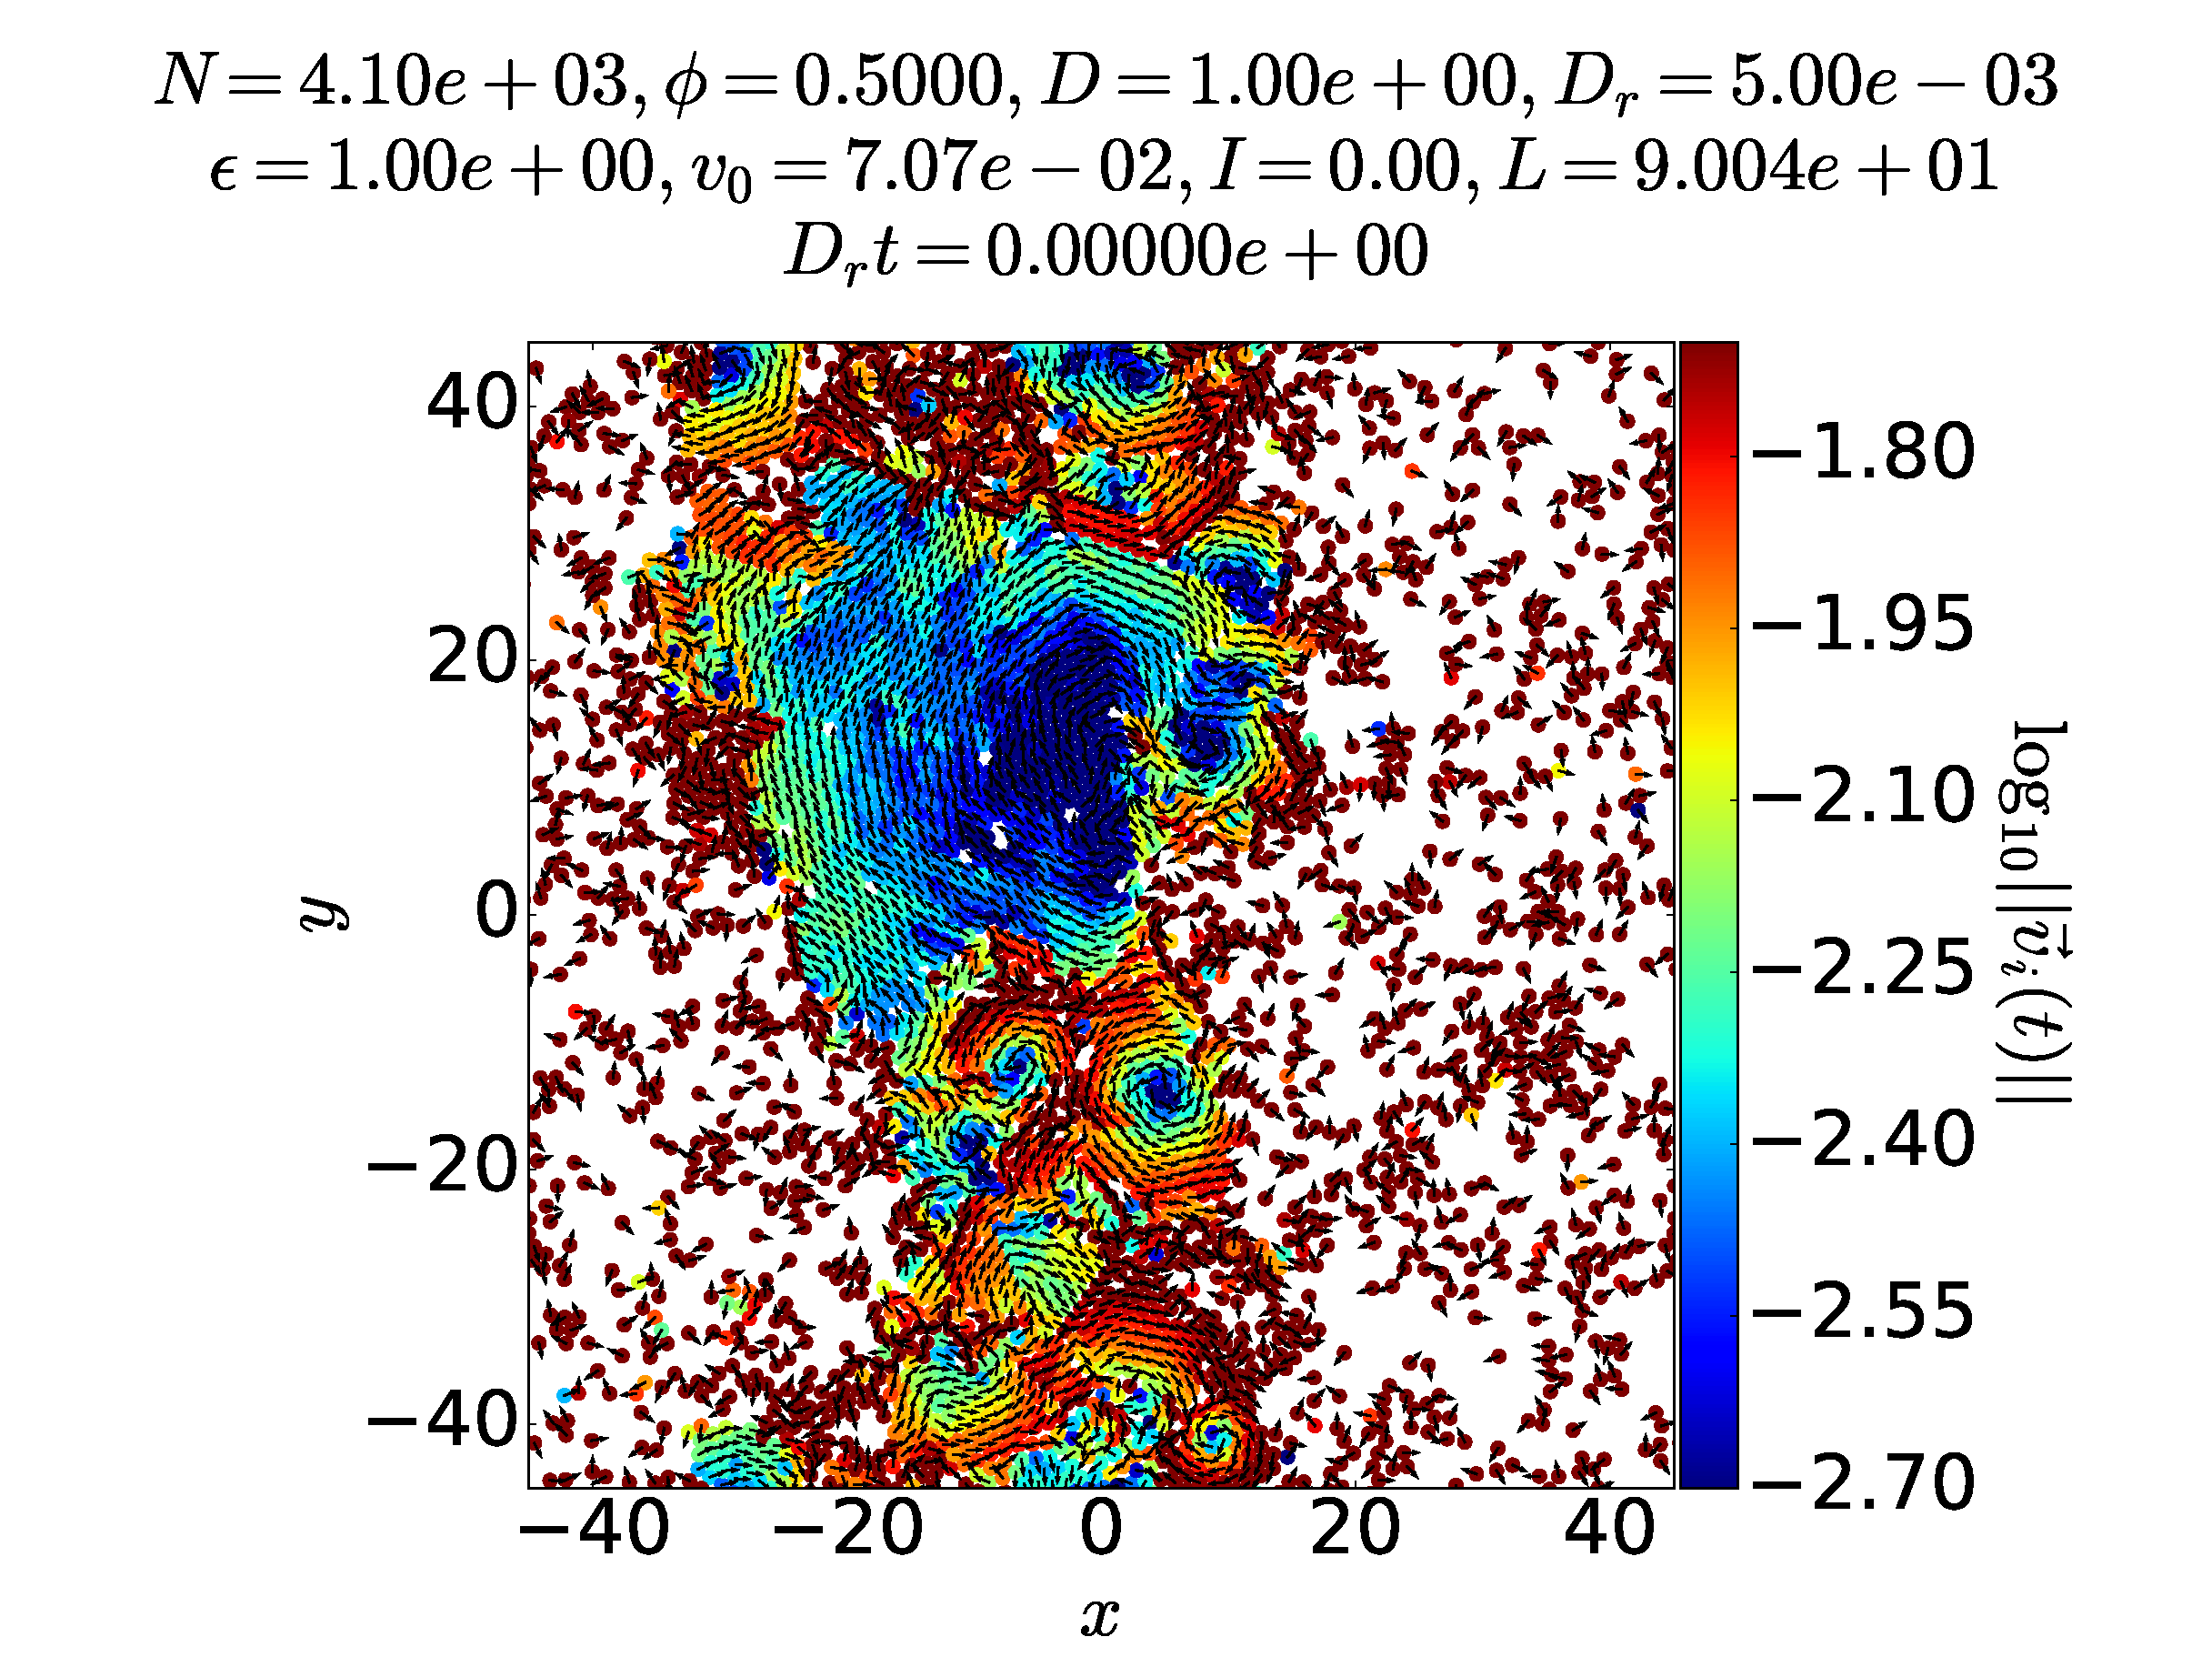
\includegraphics[width=0.45\textwidth]{No4096_Fl1000_Vl0000_Tl1000_Ri5000_Dk5000_EL3000.velo.eps}
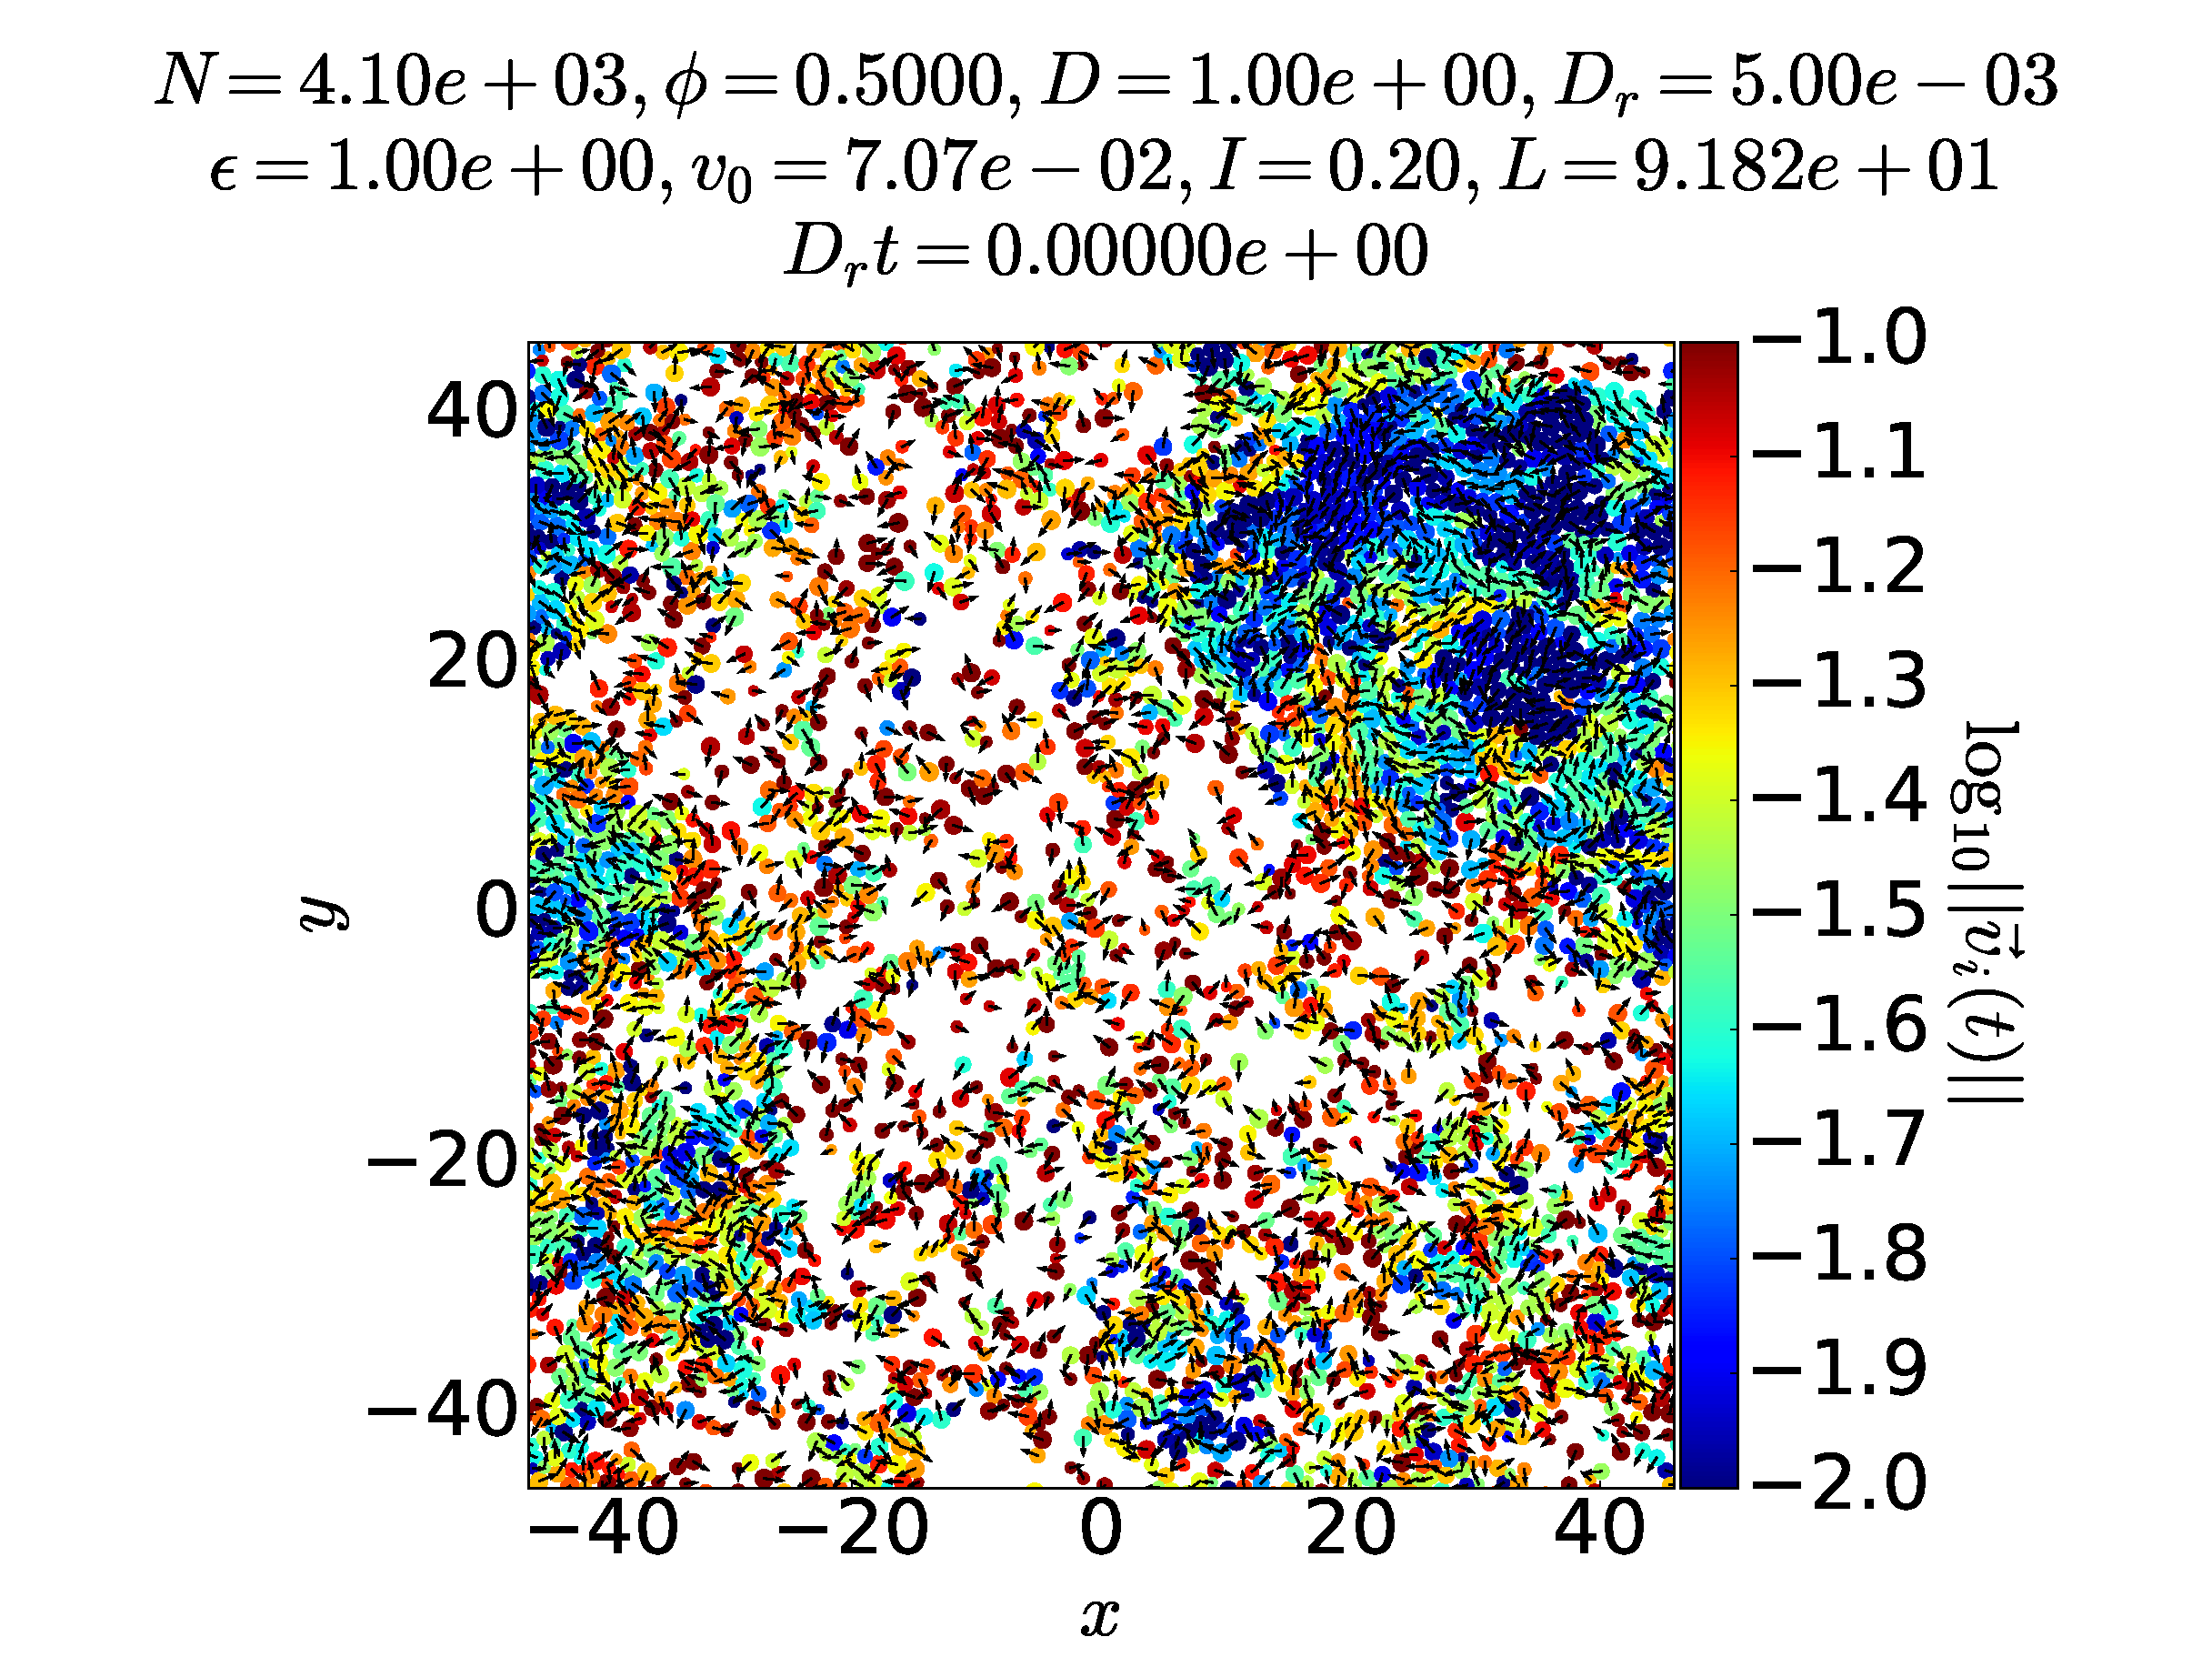
\includegraphics[width=0.45\textwidth]{No4096_Fl1000_Vl0000_Tl1000_Ri5000_Dk5000_El2000.velo.eps}
\caption{Velocity maps of AOUPs at packing fraction $\phi = 0.50$ and persistence time $\tau_p = 200$, with polydispersity index {\bf (left)} $I = 0$ {\bf (right)} $I = 0.2$.}
\end{figure}

\footfullcitenomark{martin2020statistical}
\footfullcitenomark{berthier2017active}

\end{frame}

\begin{frame}{Model}

$N$ AOUPs with evolution
\begin{eqnarray}
\dot{\boldsymbol{r}}_i = -\nabla_i U_{\rm WCA} + \boldsymbol{p}_i\\
\dot{\boldsymbol{p}}_i = - D_r \boldsymbol{p}_i + \sqrt{2 D D_r^2} \boldsymbol{\eta}_i
\end{eqnarray}
with $\left<\eta^{\alpha}_i(t)\eta^{\beta}_j(t^{\prime})\right> = \delta_{\alpha\beta} \delta_{ij} \delta(t - t^{\prime})$ such that
\begin{equation}
\left<\boldsymbol{p}_i(t) \cdot \boldsymbol{p}_j(t^{\prime})\right> = 2 \delta_{ij} D D_r e^{-D_r |t - t^{\prime}|}
\end{equation}
$l_p = \sqrt{D/D_r}$, and $\tau_p = D_r^{-1} \to 0 \equiv$ Brownian system at $T = D$.\\
\mbox{}\\

Packing fraction and polydispersity index
\begin{eqnarray}
\phi = \frac{1}{L^2} \sum_{i=1}^N \frac{\pi (\sigma_i 2^{1/6})^2}{4}\\
I = \frac{\sqrt{\left<\sigma_i^2\right> - \left<\sigma_i\right>^2}}{\left<\sigma_i\right>}
\end{eqnarray}
and we fix $I = 0.2$ from a uniform distribution.

\end{frame}

\section{Structural relaxation}

\begin{frame}{Effective diffusion constant}

\begin{figure}
\centering
\includegraphics[width=0.55\textwidth]{Deff.eps}
% \includegraphics[width=0.45\textwidth]{DeffV2.eps}
\caption{Effective diffusion constant $D_{\mathrm{eff}} = \lim_{\Delta t \to \infty} \left<|\Delta\boldsymbol{r}_i(t, t + \Delta t)|^2\right>_{i, t}/4\Delta t$.}
\end{figure}

\begin{itemize}
  \item Dramatic decrease of $D_{\rm eff}$ for small variations of $\phi$ near dynamical arrest.
\end{itemize}

\footfullcitenomark{janssen2019active}

\end{frame}

\begin{frame}{Mean squared displacement}

\begin{figure}
\centering
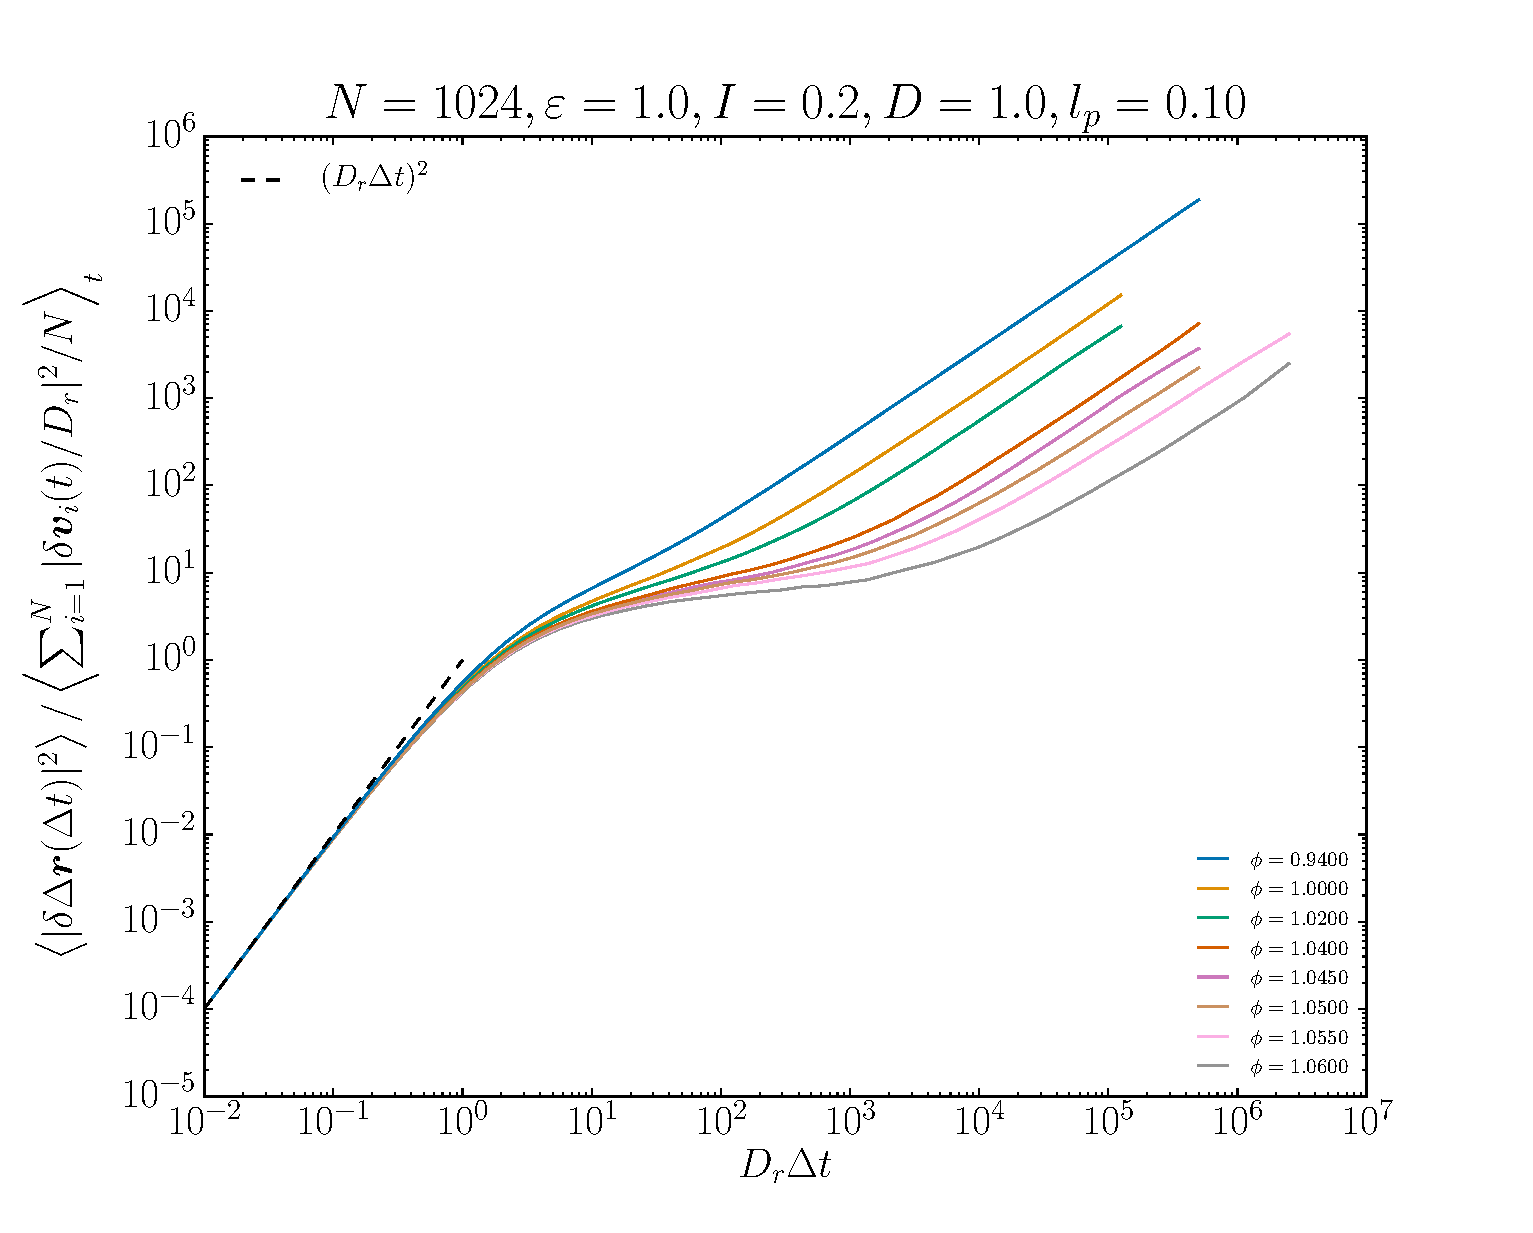
\includegraphics[width=0.45\textwidth]{msdv2_No1024_Tl1000_Rn1000.eps}
% \includegraphics[width=0.35\textwidth]{Fs_No1024_Tl1000_Rn1000.eps}\\
\includegraphics[width=0.45\textwidth]{msdv2_No1024_Tl1000_Rj1000.eps}
% \includegraphics[width=0.35\textwidth]{Fs_No1024_Tl1000_Rj1000.eps}
\caption{Mean squared displacement rescaled by mean squared velocity at {\bf (left)} $\tau_p = 10^{-2}$ and {\bf (right)} $\tau_p = 10^2$.}
\end{figure}

\begin{itemize}
  \item Significant deviation from the ballistic regime at high $\tau_p$ and smoother plateau than at low $\tau_p$.
\end{itemize}

\end{frame}

\begin{frame}{Overlap susceptibility}

\begin{equation}
\chi(\Delta t, a) = N \mathrm{Var}\left(\exp\left(-|\Delta \boldsymbol{r}_i(t, t + \Delta t)|^2/a^2\right)\right)_t
\end{equation}
\mbox{}\\

\begin{figure}
\centering
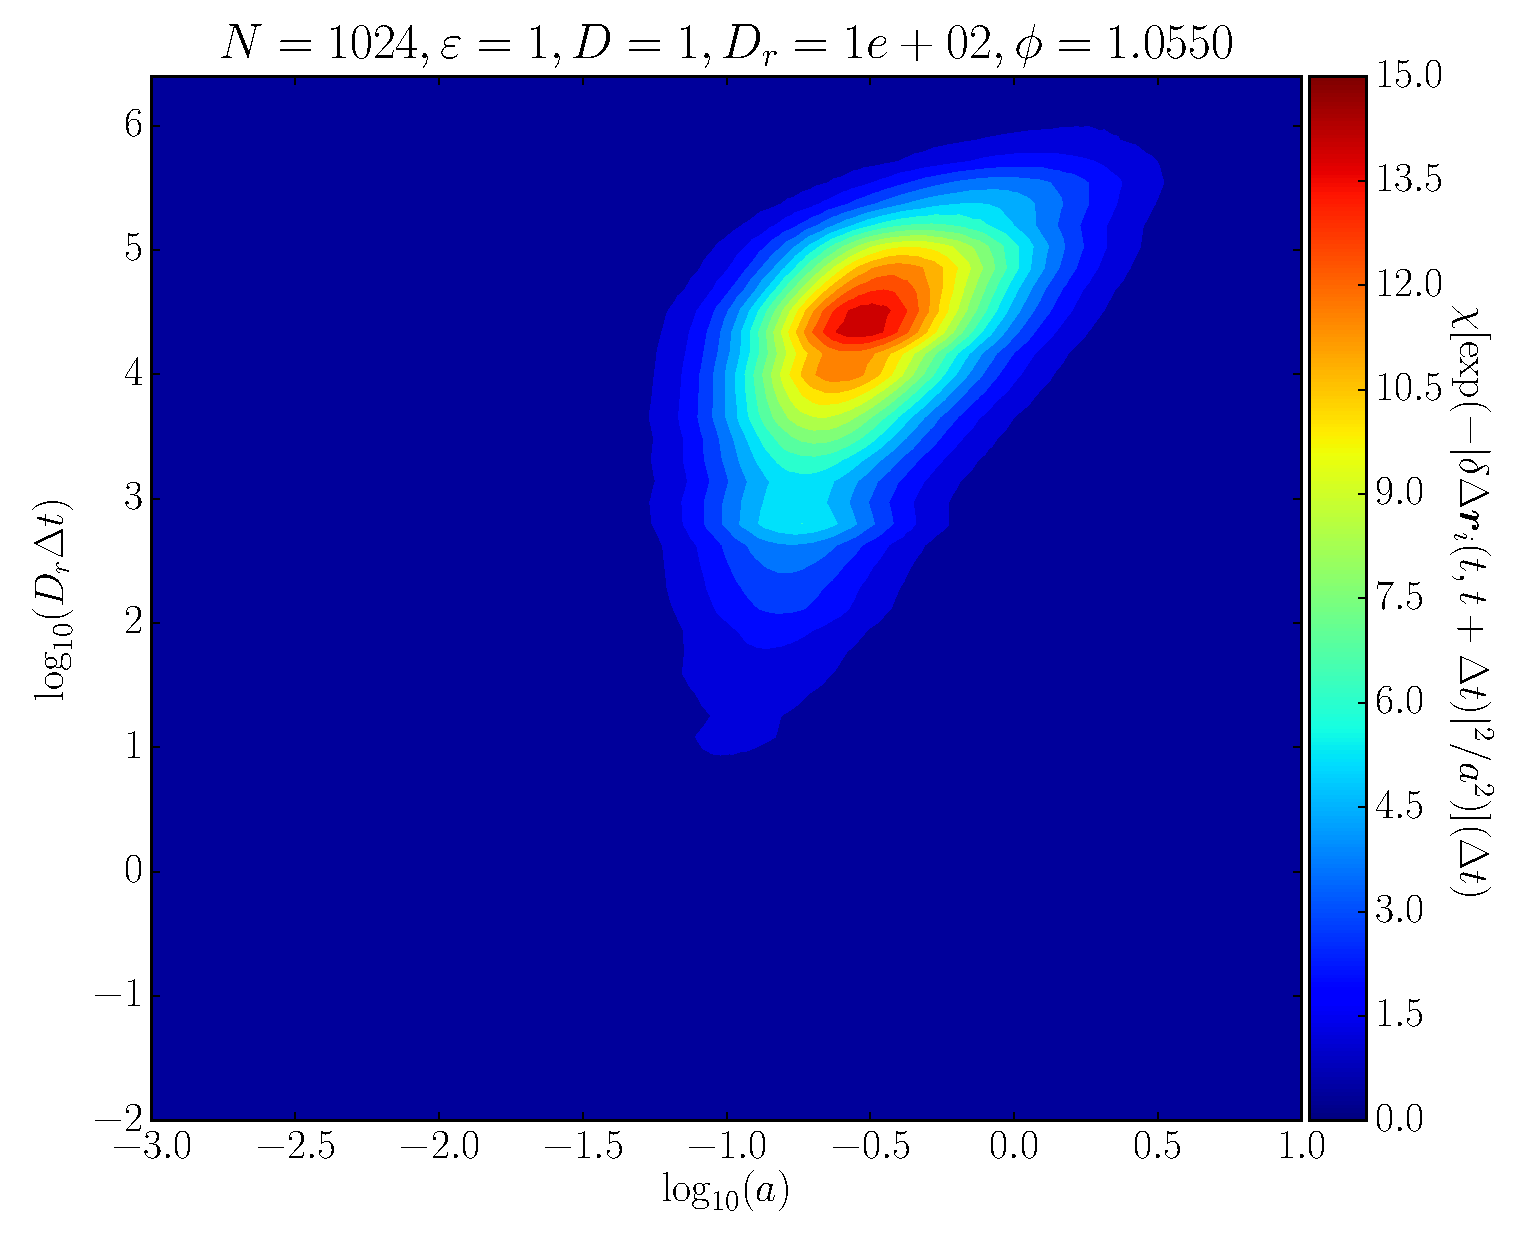
\includegraphics[width=0.45\textwidth]{No1024_Fl1000_Vl0000_Tl1000_Rn1000_Dl1055_El0000.datN.overlap.eps}
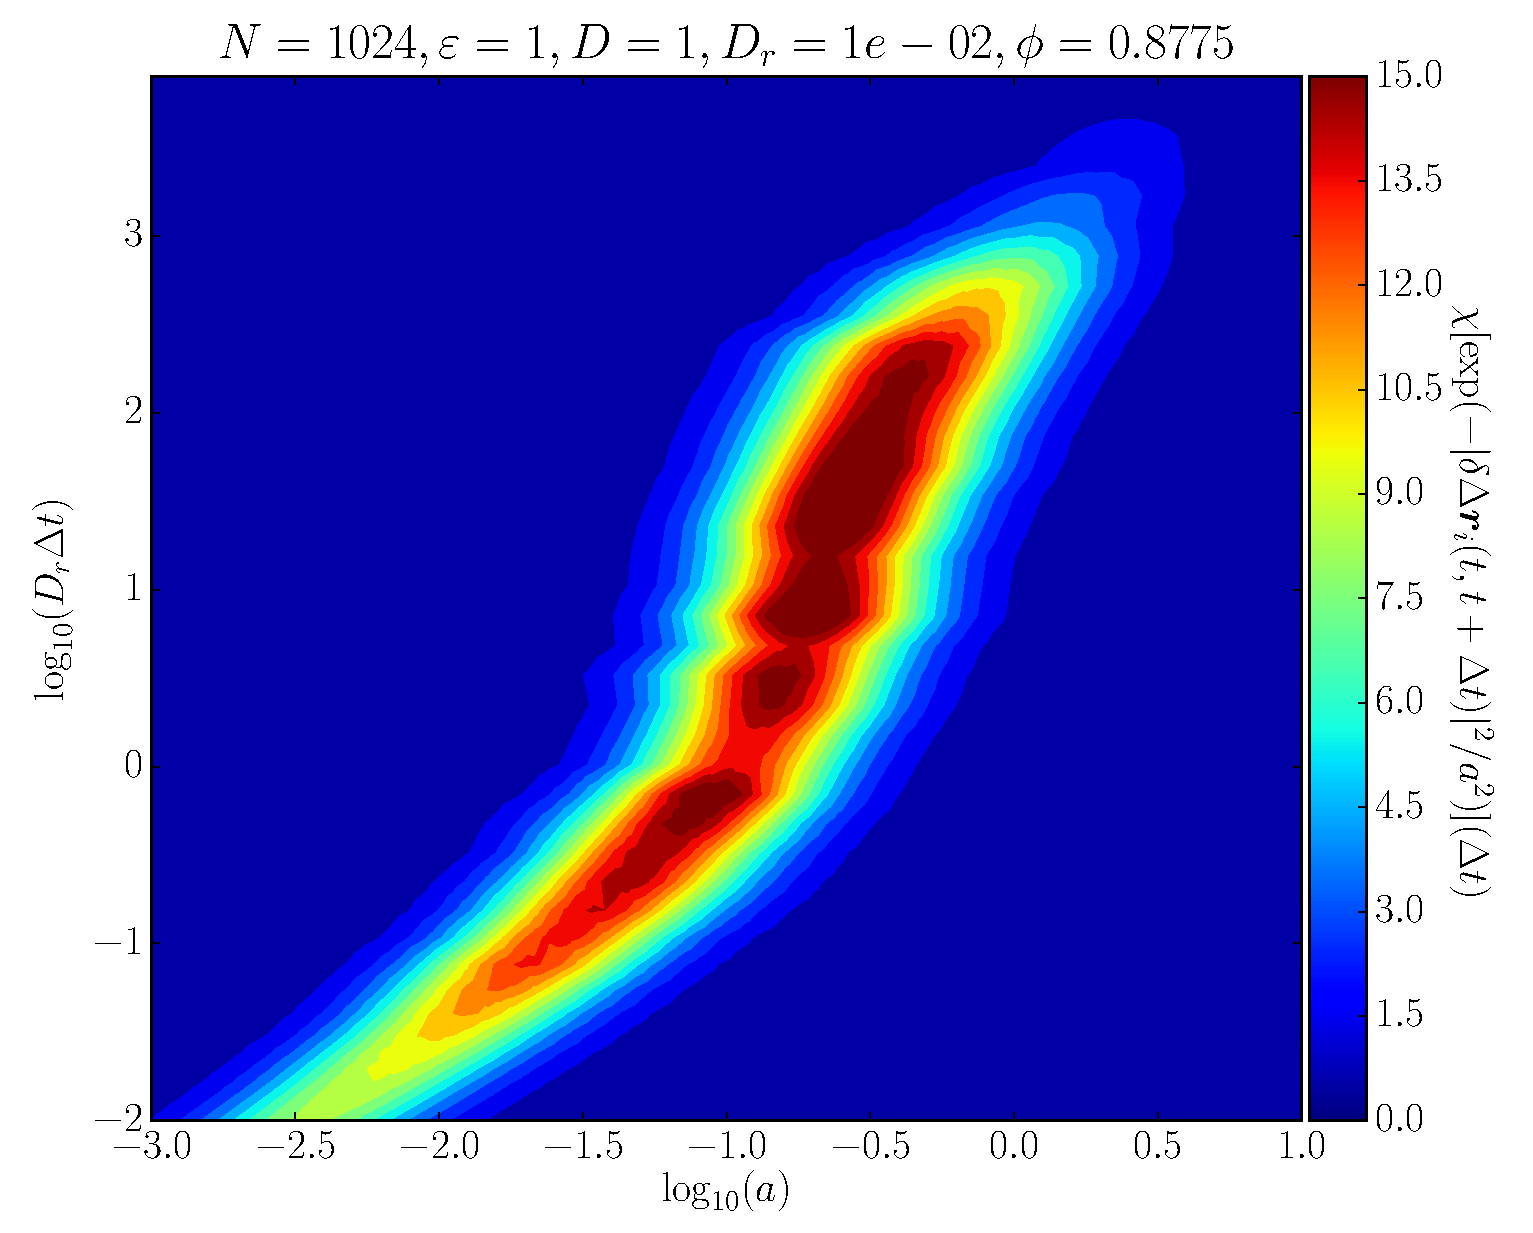
\includegraphics[width=0.45\textwidth]{No1024_Fl1000_Vl0000_Tl1000_Rj1000_Dk8775_El0000.datN.overlap.eps}
\caption{Overlap susceptibility $\chi$ at {\bf (left)} $\tau_p = 10^{-2}$ and {\bf (right)} $\tau_p = 10^2$.}
\end{figure}

\begin{itemize}
  \item Large dynamical heterogeneities at time scales significantly lower than relaxation time for high $\tau_p$.
\end{itemize}

\end{frame}

\section{Velocity correlations}

\begin{frame}{Velocity maps}

\begin{figure}
\centering
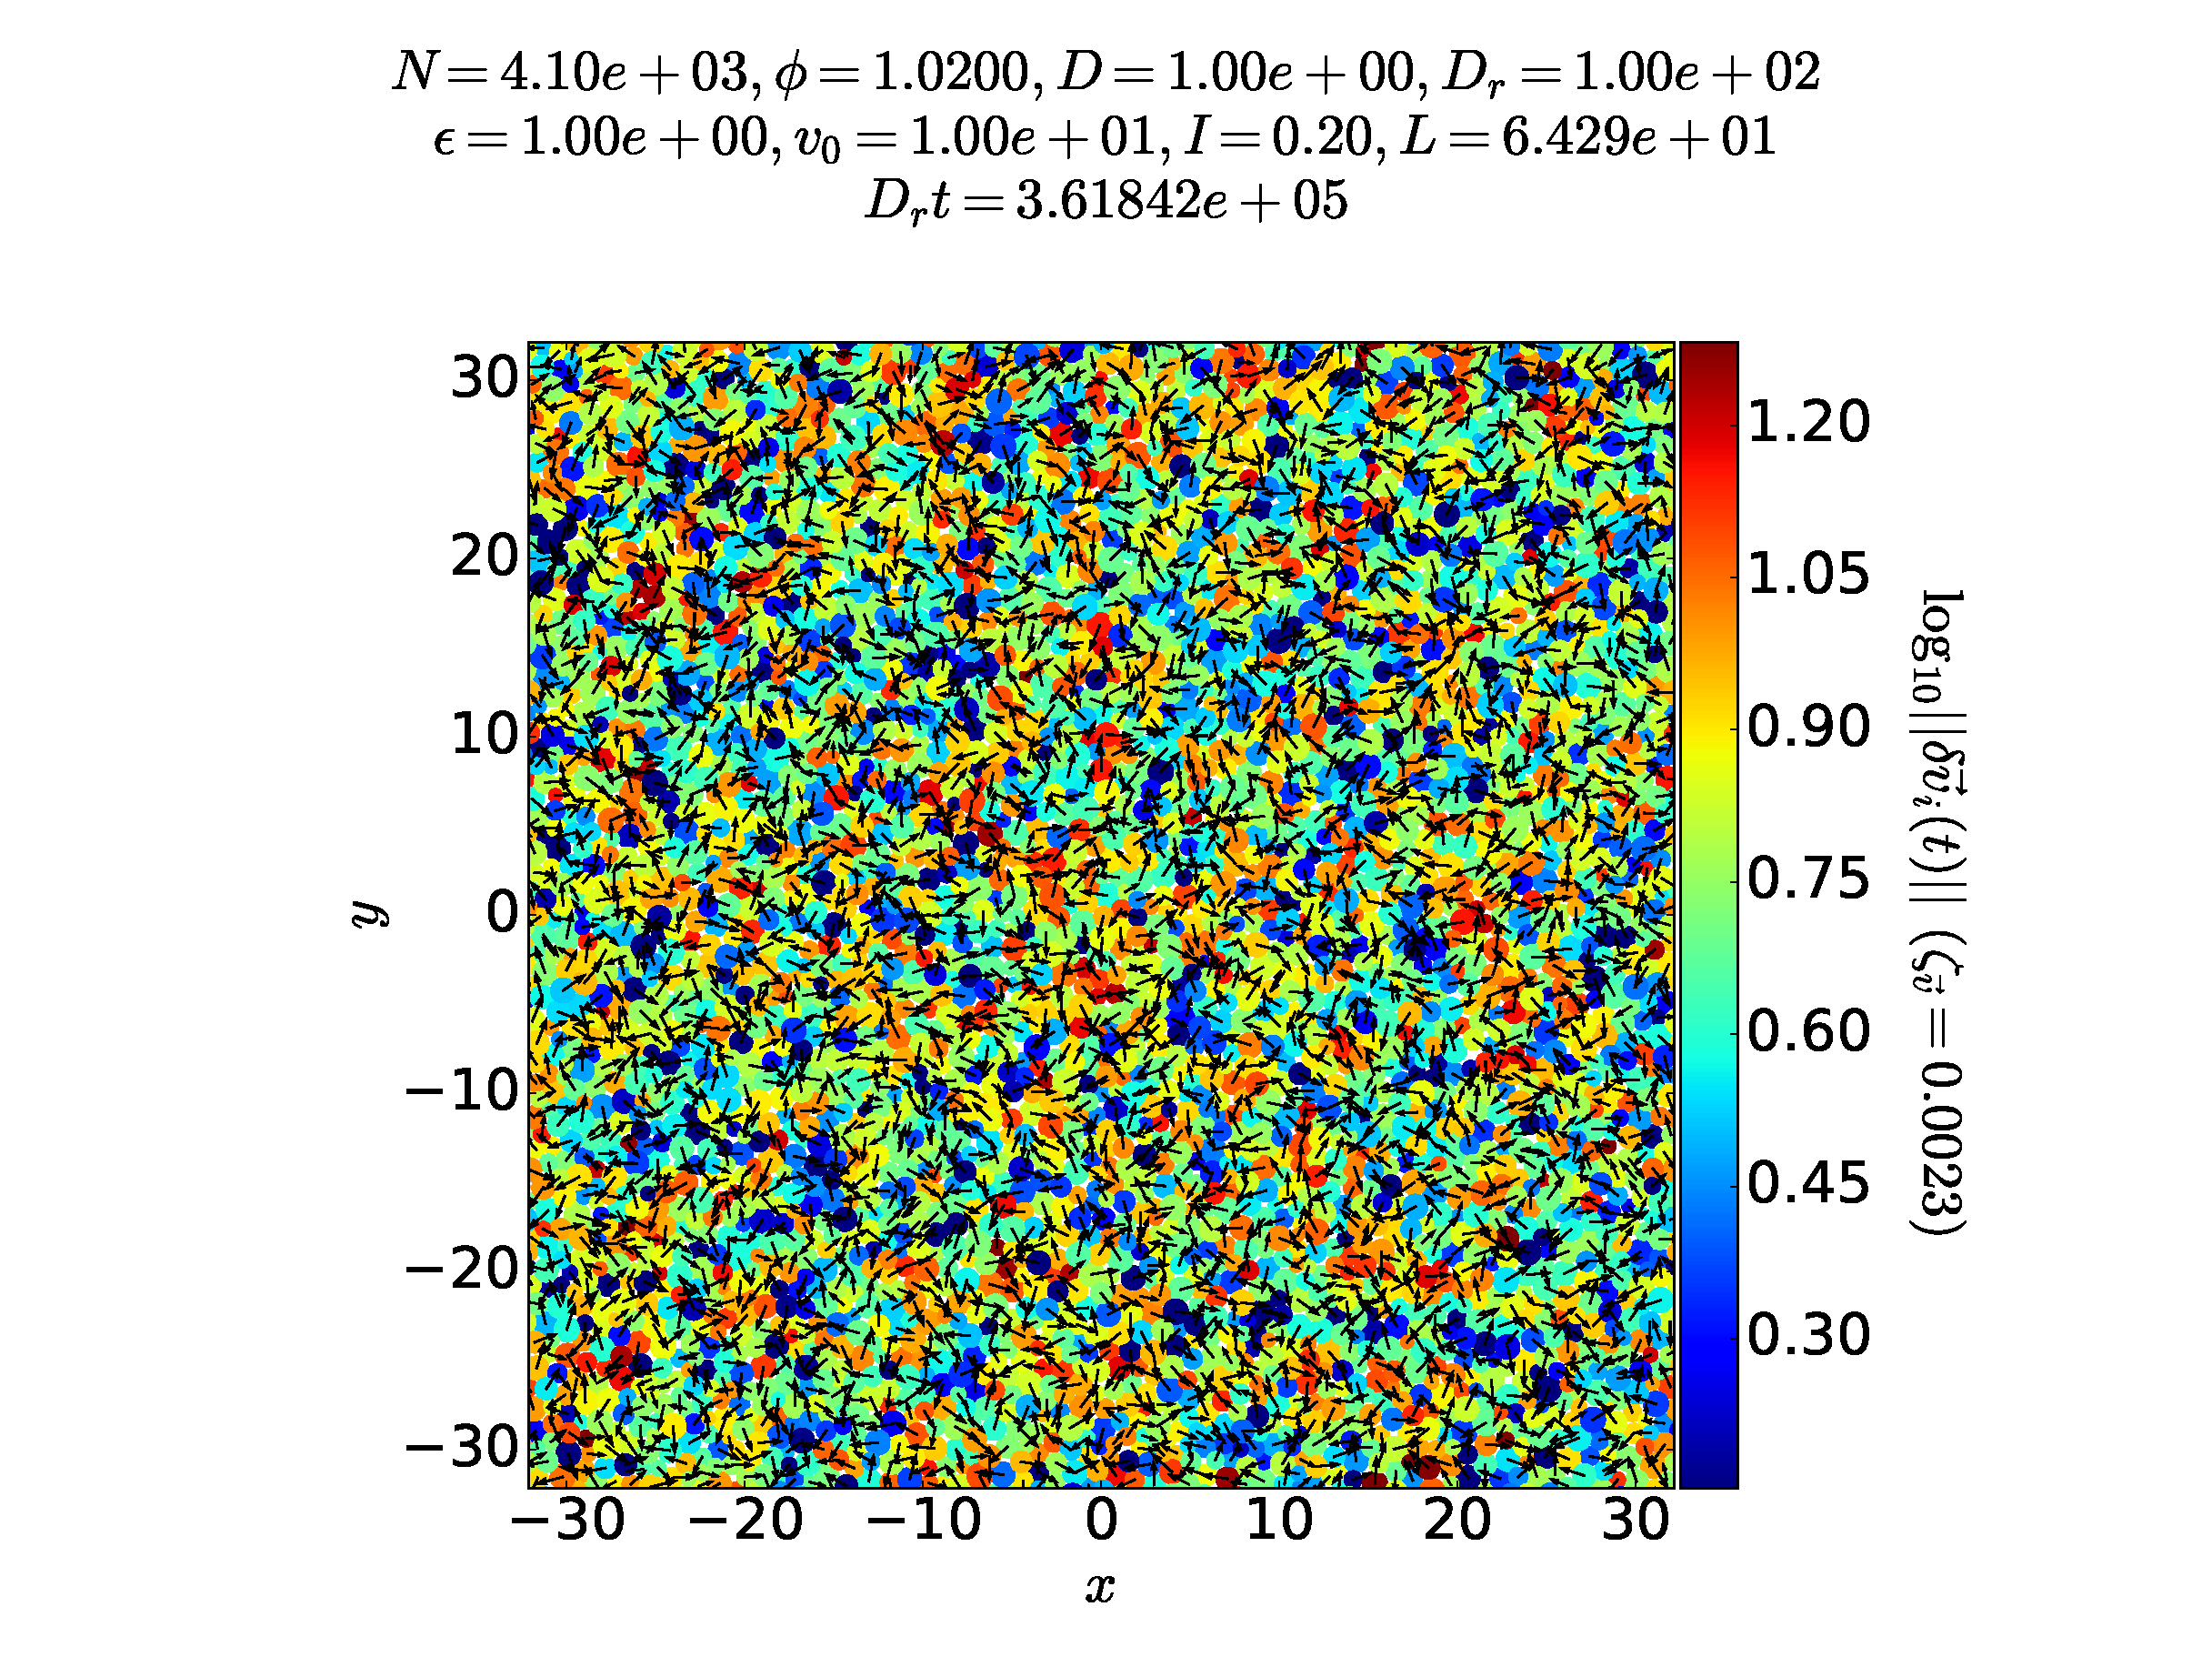
\includegraphics[width=0.49\textwidth]{No4096_Fl1000_Vl0000_Tl1000_Rn1000_Dl1020_El0000.velo.eps}
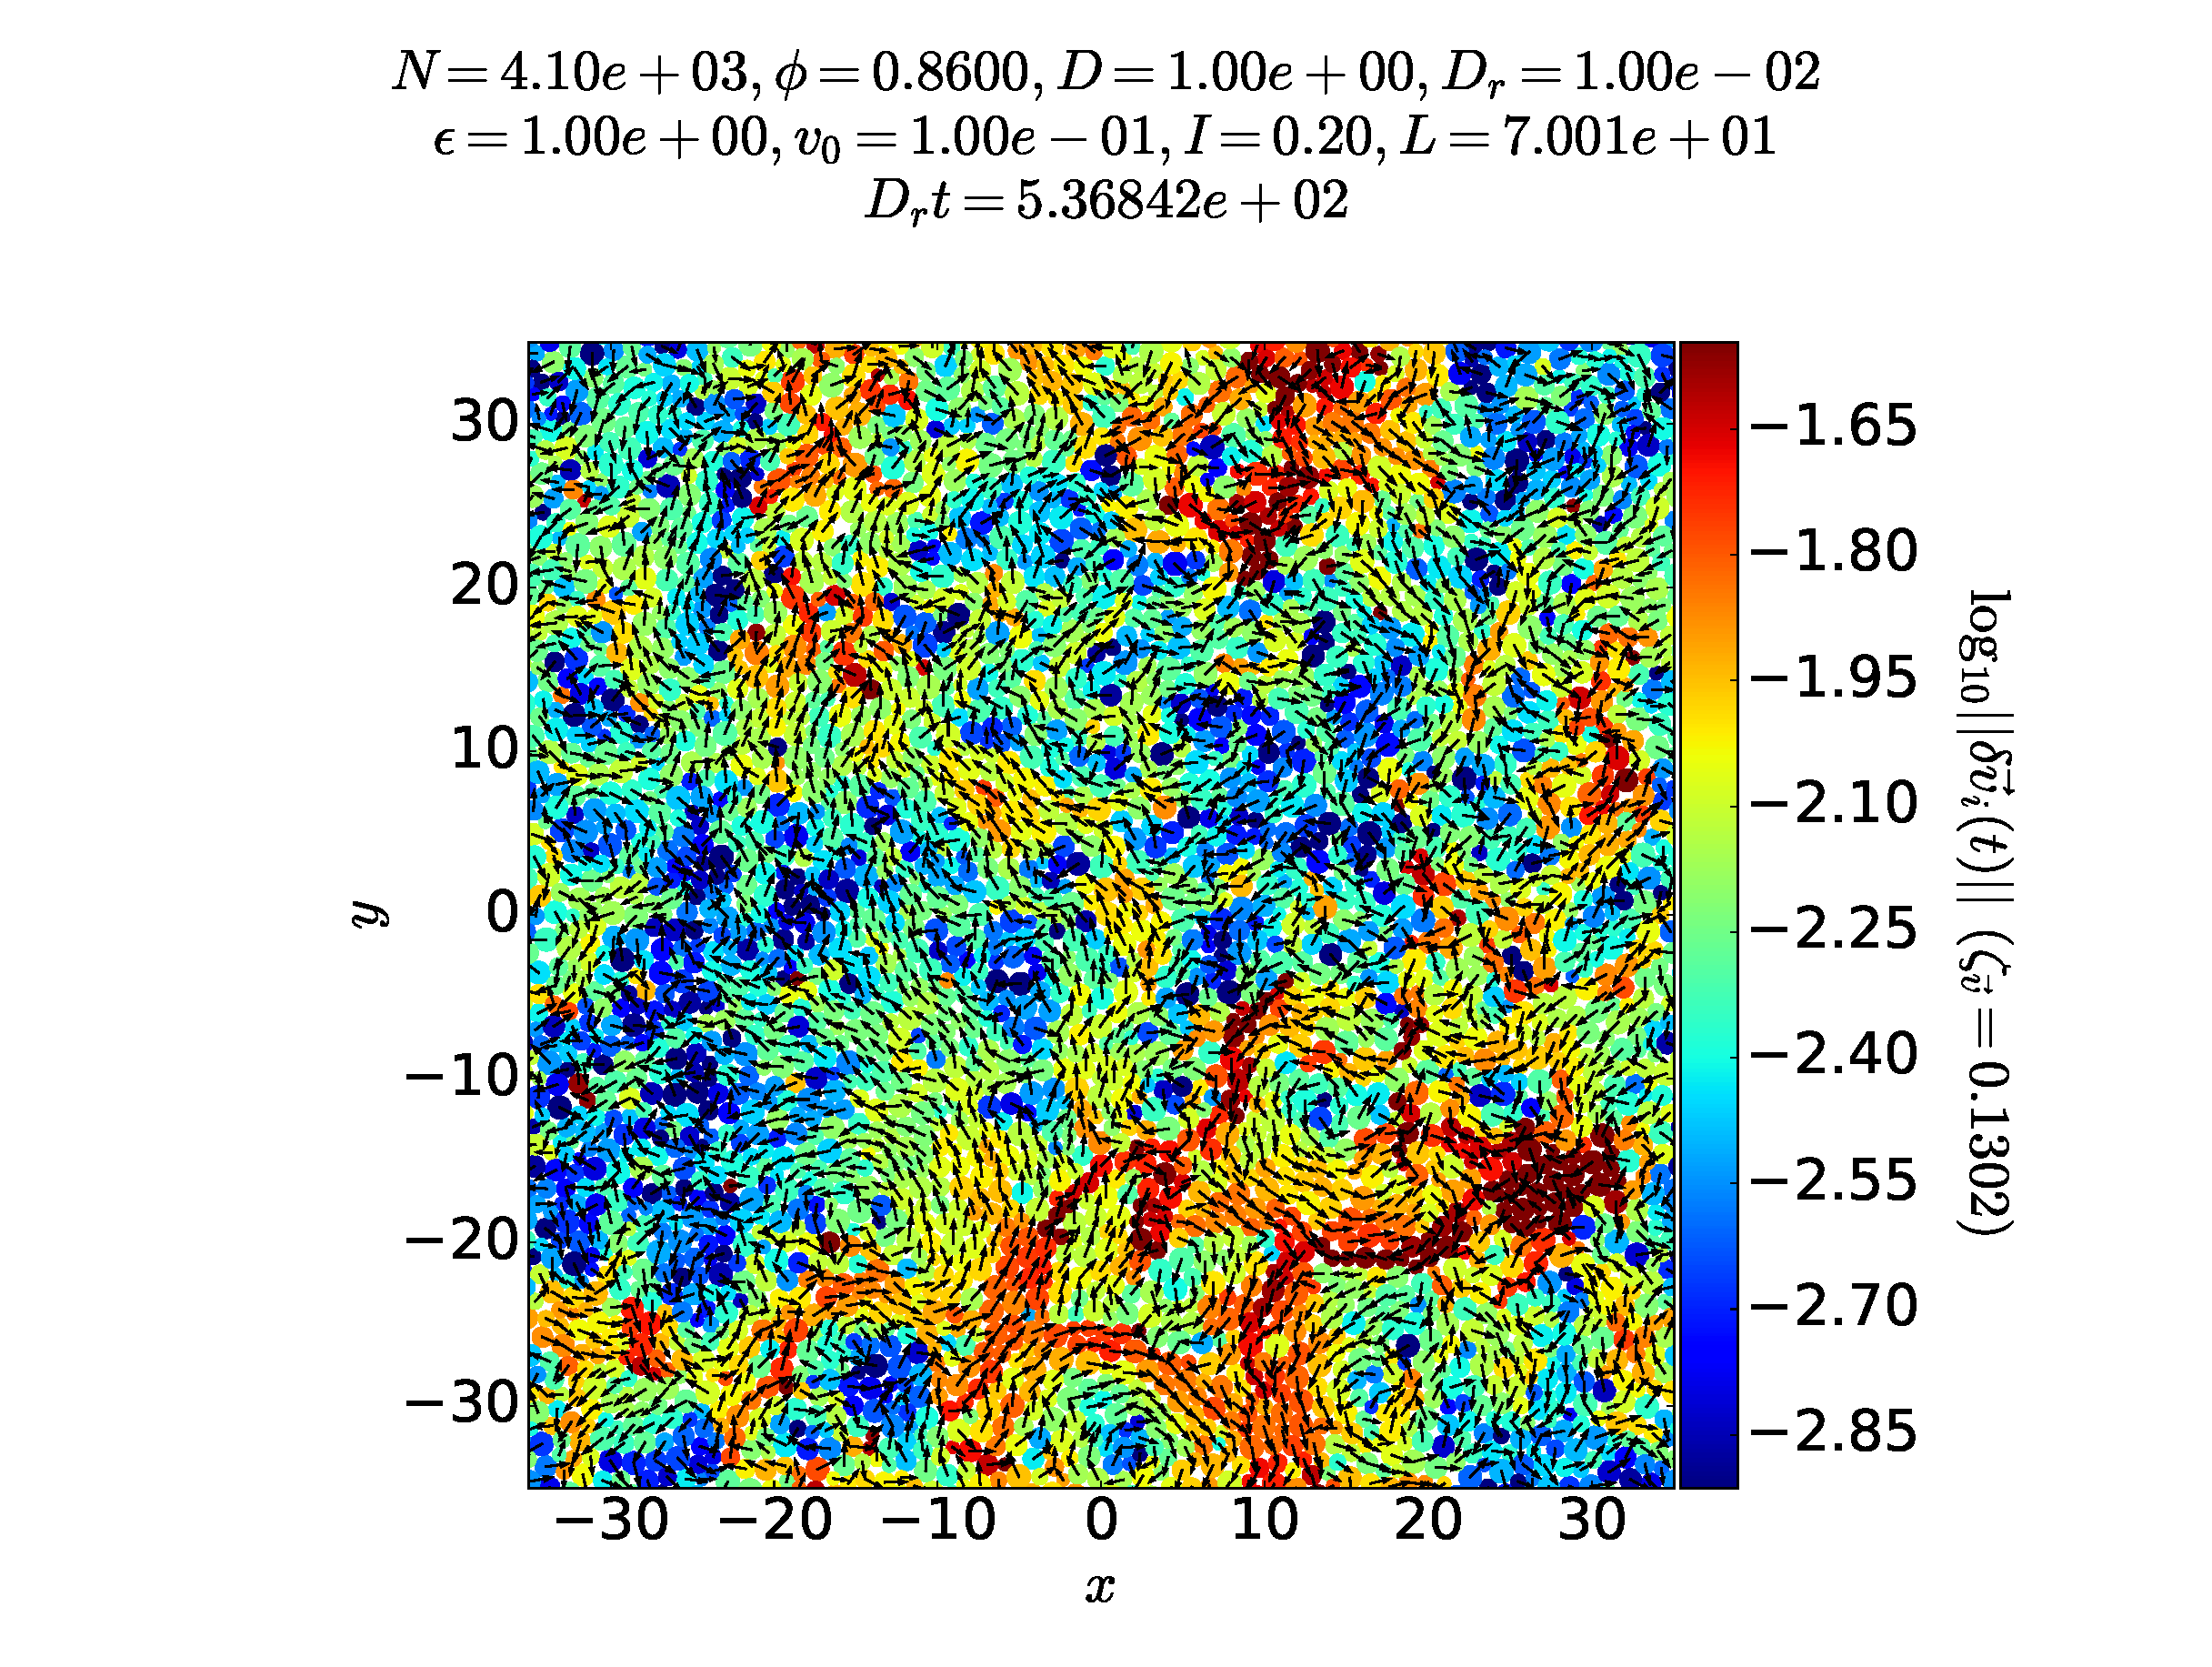
\includegraphics[width=0.49\textwidth]{No4096_Fl1000_Vl0000_Tl1000_Rj1000_Dk8600_El0000.velo.eps}
\caption{Velocity maps at {\bf (left)} $\tau_p = 10^{-2}$ and {\bf (right)} $\tau_p = 10^2$.}
\end{figure}

\begin{itemize}
  \item Large $\tau_p$ associated with multiparticle scale velocity correlations.
\end{itemize}

\footfullcitenomark{caprini2020hidden}

\end{frame}

\begin{frame}{Velocity radial correlations}

\begin{figure}
\centering
\includegraphics[width=0.45\textwidth]{cvvCMlog_No1024_Tl1000_Rn1000.eps}
\includegraphics[width=0.45\textwidth]{cvvCMlog_No1024_Tl1000_Rj1000.eps}
\caption{Velocity radial autocorrelation function at {\bf (left)} $\tau_p = 10^{-2}$ and {\bf (right)} $\tau_p = 10^2$.}
\end{figure}

\begin{itemize}
  \item Velocity correlation length increases with both $\tau_p$ and $\phi$.
\end{itemize}

\end{frame}

\begin{frame}{Velocity temporal correlations}

\begin{figure}
\centering
\includegraphics[width=0.45\textwidth]{cvvtCM_No1024_Tl1000_Rn1000.eps}
\includegraphics[width=0.45\textwidth]{cvvtCM_No1024_Tl1000_Rj1000.eps}
\caption{Velocity temporal autocorrelation function at {\bf (left)} $\tau_p = 10^{-2}$ and {\bf (right)} $\tau_p = 10^2$.}
\end{figure}

\begin{itemize}
  \item Velocity correlation time decreases with $\phi$ but remains approximately of the order of $\tau_p$.
\end{itemize}

\end{frame}

\begin{frame}{Velocity distribution}

\begin{figure}
\centering
% \includegraphics[width=0.35\textwidth]{No1024_Fl1000_Vl0000_Tl1000_Rn1000.pvx.eps}
\includegraphics[width=0.45\textwidth]{No1024_Fl1000_Vl0000_Tl1000_Rn1000.pv2.eps}
% 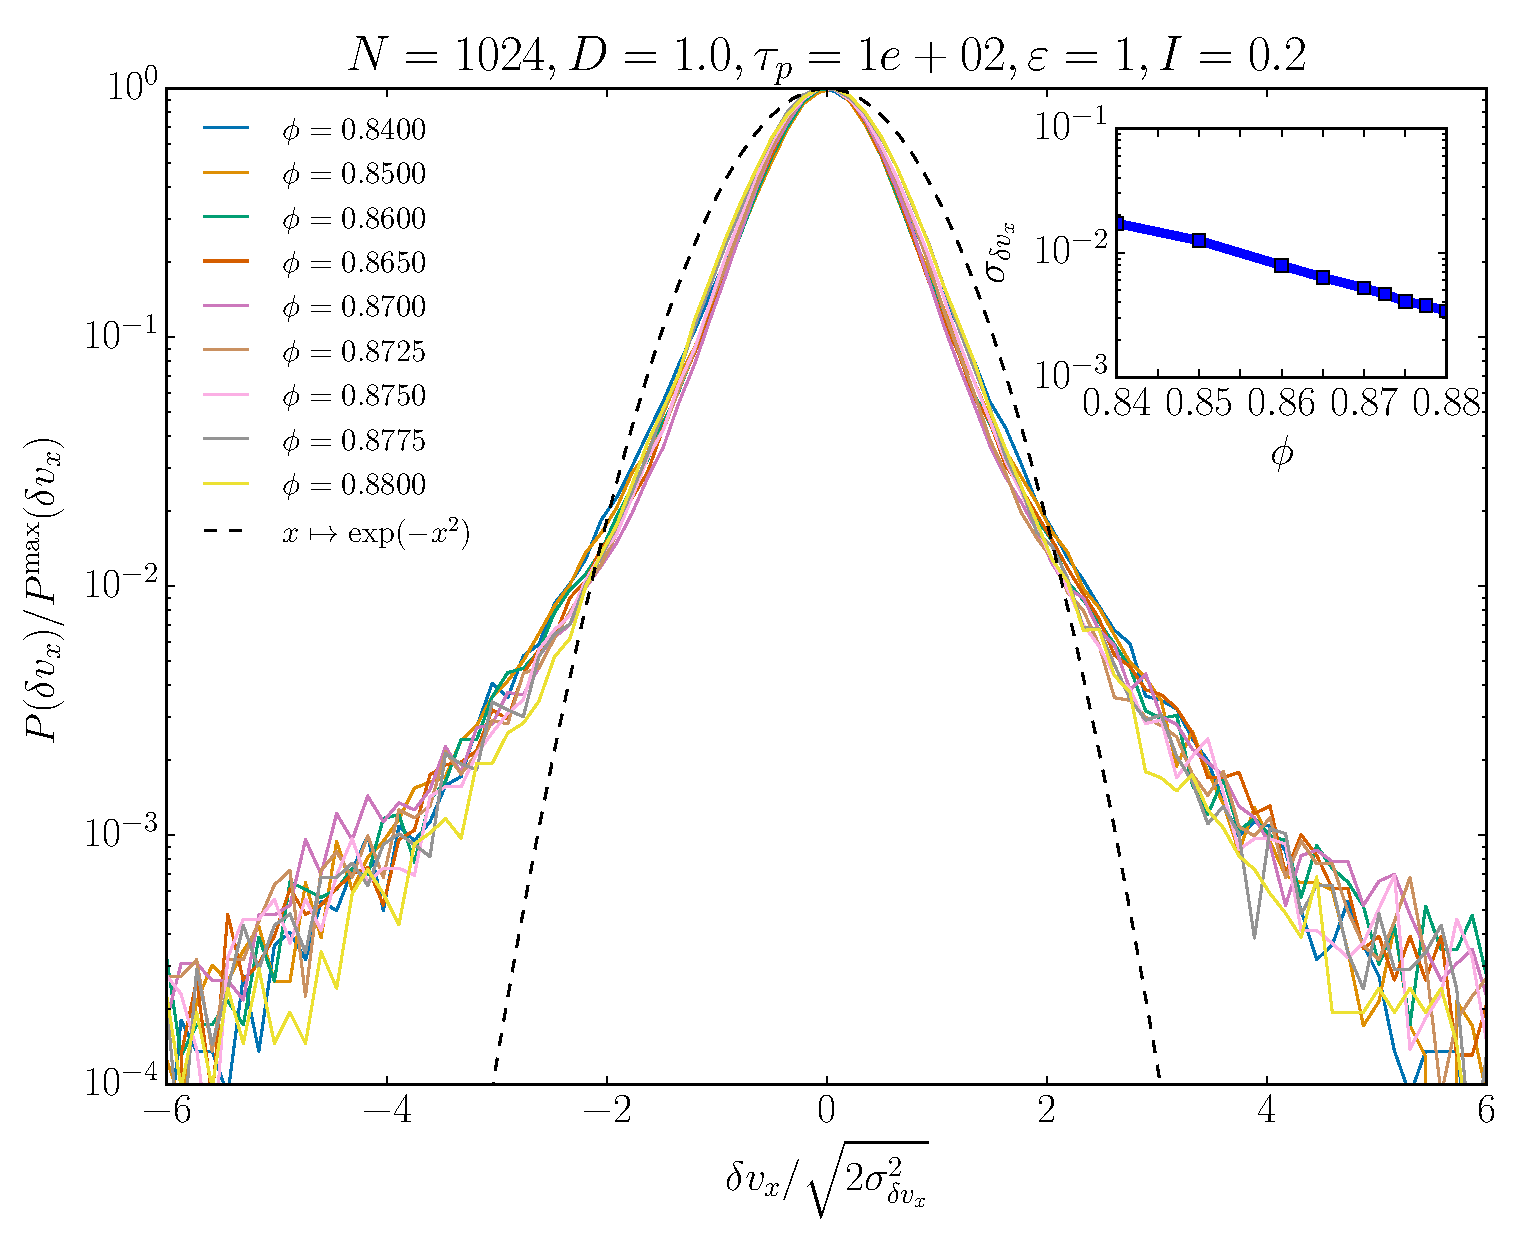
\includegraphics[width=0.35\textwidth]{No1024_Fl1000_Vl0000_Tl1000_Rj1000.pvx.eps}
\includegraphics[width=0.45\textwidth]{No1024_Fl1000_Vl0000_Tl1000_Rj1000.pv2.eps}
\caption{Distributions of $|\boldsymbol{v}|^2$ at {\bf (left)} $\tau_p = 10^{-2}$ and {\bf (right)} $\tau_p = 10^2$.}
\end{figure}

\begin{itemize}
  \item At low $\tau_p$, the distribution of $|\boldsymbol{v}|^2$ remains approximately Gaussian, and $|\boldsymbol{v}|^2 = \mathcal{O}(D D_r)$ the injected energy.
  \item At high $\tau_p$, $|\boldsymbol{v}|^2$ distribution has a fat tail and $|\boldsymbol{v}|^2 \ll \mathcal{O}(D D_r)$ indicating $-\nabla_i U_{\rm WCA} \approx -\boldsymbol{p}_i$.
\end{itemize}

\footfullcitenomark{caprini2020active}

\end{frame}

\begin{frame}{Time series of kinetic energy}

\begin{figure}
\centering
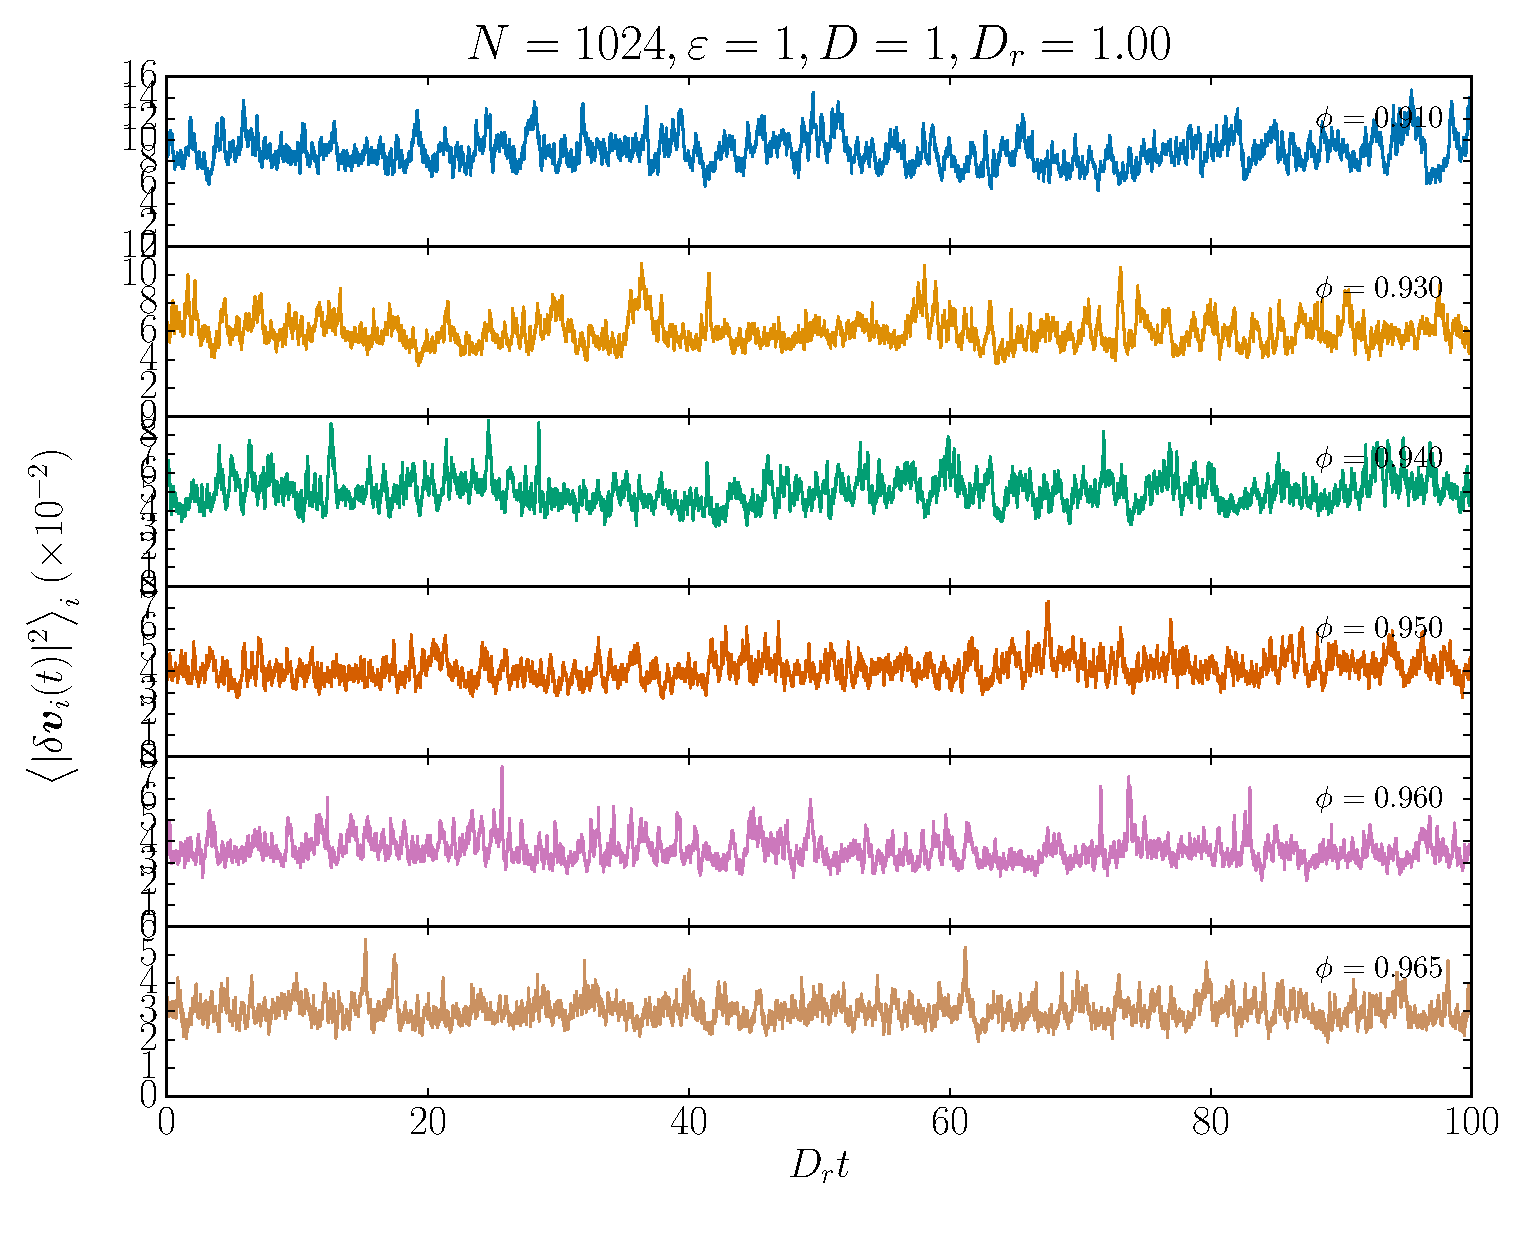
\includegraphics[width=0.45\textwidth]{No1024_Fl1000_Vl0000_Tl1000_Rl1000.ecC.eps}
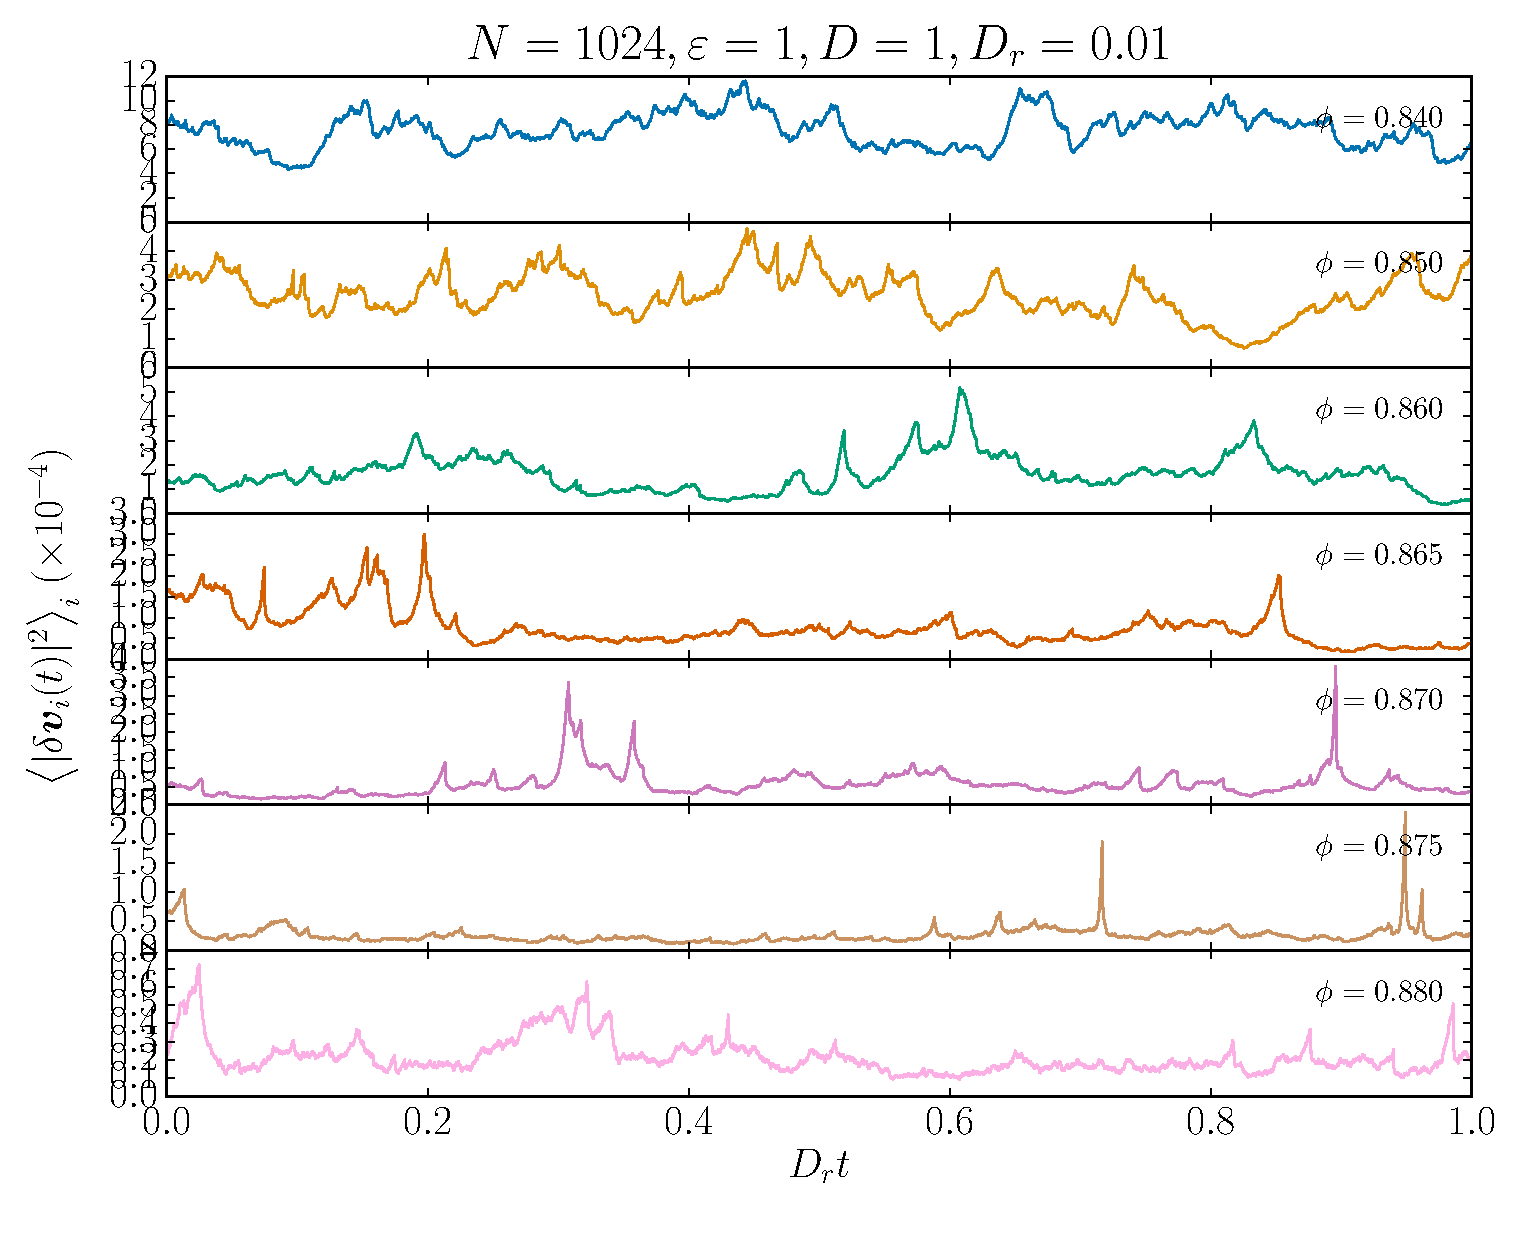
\includegraphics[width=0.45\textwidth]{No1024_Fl1000_Vl0000_Tl1000_Rj1000.ecC.eps}
\caption{Time series of kinetic energy at {\bf (left)} $\tau_p = 10^0$ and {\bf (right)} $\tau_p = 10^2$.}
\end{figure}

\begin{itemize}
  \item At high $\tau_p$ and $\phi$, $|\boldsymbol{v}|^2$ is intermittent signaling plastic yielding events between force-balanced $(\boldsymbol{r}_i, \boldsymbol{p}_i)$ configurations.
\end{itemize}

\footfullcitenomark{mandal2020extreme}
\footfullcitenomark{caprini2020active}

\end{frame}

\section{Outlook}

\begin{frame}{Tentative phase diagram}

\begin{figure}
\centering
\includegraphics[height=4cm]{mandal2020_fig1a.png}
\includestandalone[height=4cm]{diagram}
\caption{{\bf (left)} Phase diagram for ABPs at fixed $\phi$ with $f \sim \sqrt{D D_r}$ \FigureFrom{mandal2020extreme}{1(a)}. {\bf (right)} Provisional phase diagram for AOUPs at fixed $D$.}
\end{figure}

At fixed D,
\begin{itemize}
  \item the system is equilibrium-like for $l_p$ smaller than cage size,
  \item large cooperative motion is possible at intermediate $\phi$ and $\tau_p$ but is hindered by increasing $\phi$ or $\tau_p$ leading to force-balanced states.
\end{itemize}

\end{frame}

{
\footerwithoutframenumber

\begin{frame}[noframenumbering]{Theoretical velocity correlations}

\begin{figure}
\centering
\includegraphics[height=2.75cm]{henkes2020_fig1a.png}
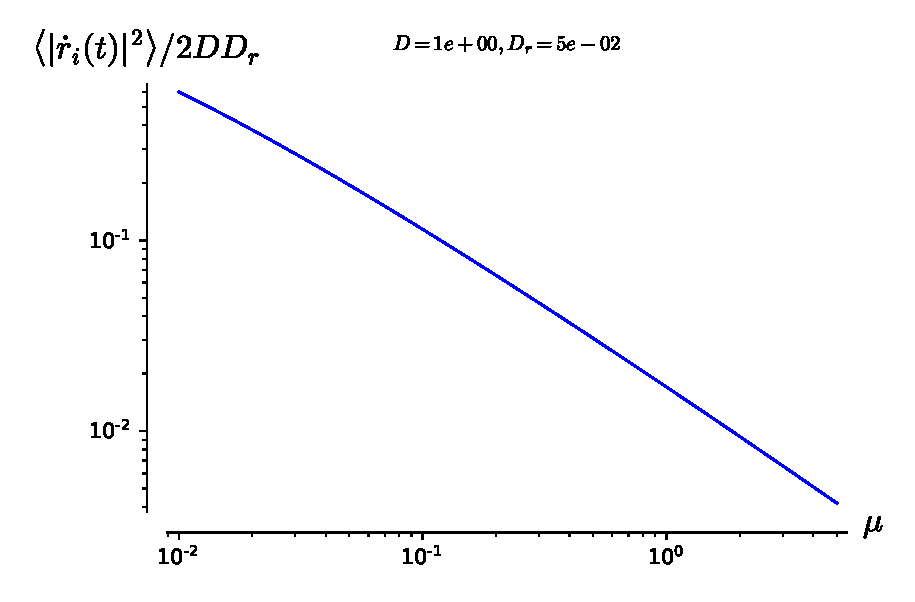
\includegraphics[height=2.75cm]{henkes_natcomm_2020_eq11.eps}
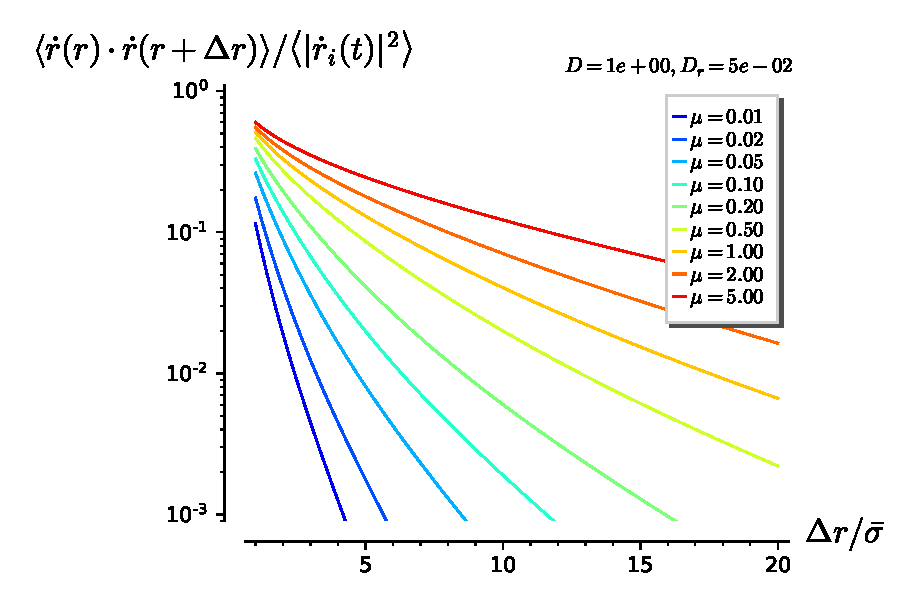
\includegraphics[height=2.75cm]{henkes_natcomm_2020_eq62.eps}\\
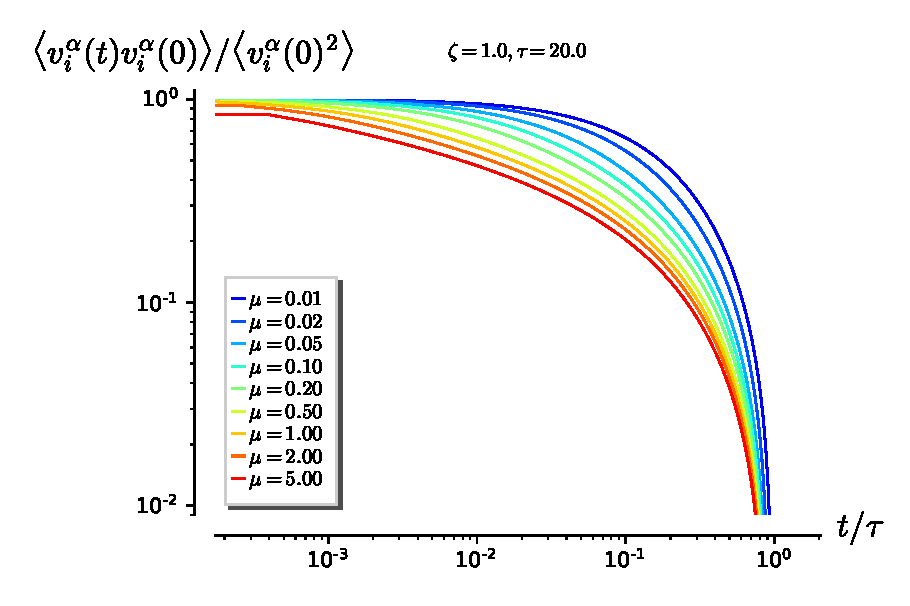
\includegraphics[height=2.75cm]{henkes_natcomm_2020_eq57.eps}
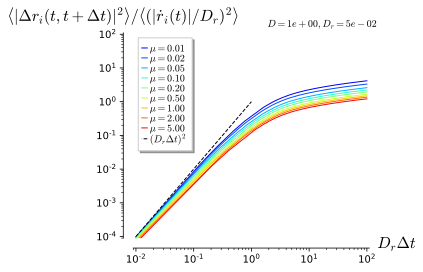
\includegraphics[height=2.75cm]{henkes_natcomm_2020_eq57_msd.eps}
\caption{{\bf (top left)} Active elastic theory \FigureFrom{henkes2020dense}{1(a)}. {\bf (top centre)} Mean squared velocity. {\bf (top right)} Radial autocorrelation function of velocity. {\bf (bottom left)} Temporal autocorrelation of velocity. {\bf (bottom right)} Mean squared displacement.}
\end{figure}

\vspace{-10pt}
\footfullcitenomark{szamel2021long}

\end{frame}

\begin{frame}[noframenumbering]{Pair distribution function}

\begin{figure}
\centering
\includegraphics[width=0.45\textwidth]{g_No1024_Tl1000_Rn1000.eps}
% \includegraphics[width=0.35\textwidth]{S_No1024_Tl1000_Rn1000.eps}\\
\includegraphics[width=0.45\textwidth]{g_No1024_Tl1000_Rj1000.eps}
% \includegraphics[width=0.35\textwidth]{S_No1024_Tl1000_Rj1000.eps}
\caption{Diameter-relative pair distribution function $g_{\sigma}$ at {\bf (left)} $\tau_p=10^{-2}$ and {\bf (right)} $\tau_p = 10^2$.}
\end{figure}

\begin{itemize}
  \item Increasing effective radius of particles with increasing $\tau_p$, consistent with decreasing $D_{\rm eff}$.
  \item Sharpening and growth of the first peak (increasing adhesion) is a general feature of self-propelled particles.
\end{itemize}

\footfullcitenomark{berthier2017active}

\end{frame}

\begin{frame}[noframenumbering]{Swim velocity}

\begin{equation}
v(\rho)/\left<|\boldsymbol{p}_i|\right> = 1 + \left<-\nabla_i U \cdot \boldsymbol{p}_i/|\boldsymbol{p}_i|\right>
\end{equation}

\begin{figure}
\centering
\includegraphics[width=0.30\textwidth]{fo_No1024_Tl1000_Rj1000.eps}
\includegraphics[width=0.30\textwidth]{fo_No1024_Tl1000_Rk1000.eps}\\
\includegraphics[width=0.30\textwidth]{fo_No1024_Tl1000_Rl1000.eps}
\includegraphics[width=0.30\textwidth]{fo_No1024_Tl1000_Rn1000.eps}
\caption{Rescaled swim velocity.}
\end{figure}

\vspace{-10pt}
\footfullcitenomark{solon2015pressure}

\end{frame}

}

\end{document}
